\documentclass[floatfix,aps,prd,amsmath,amssymb]{revtex4}

\usepackage{hyperref}
\usepackage{epsfig}
\usepackage{color}
\usepackage{graphicx}
\usepackage{float}
\usepackage{listing} %listings
\usepackage{braket}
\usepackage{mathtools}
\usepackage[noabbrev,capitalise]{cleveref} %for \cref in CKM-Mechanism.tex 
\providecommand{\e}[1]{\ensuremath{\times 10^{#1}}} %because my scientific notation wouldn't work: Kevin
\usepackage{tensor}
\usepackage{amsmath}

\begin{document}
\title{The Lorentz Group and Singular Lorentz Transformations}
\author{Kevin Maguire (10318135)}
\date{\today}

\begin{abstract}
\textit{abstract}
\end{abstract}

\maketitle
\pagenumbering{roman}

%\begin{figure}[h!]
%\begin{center}
%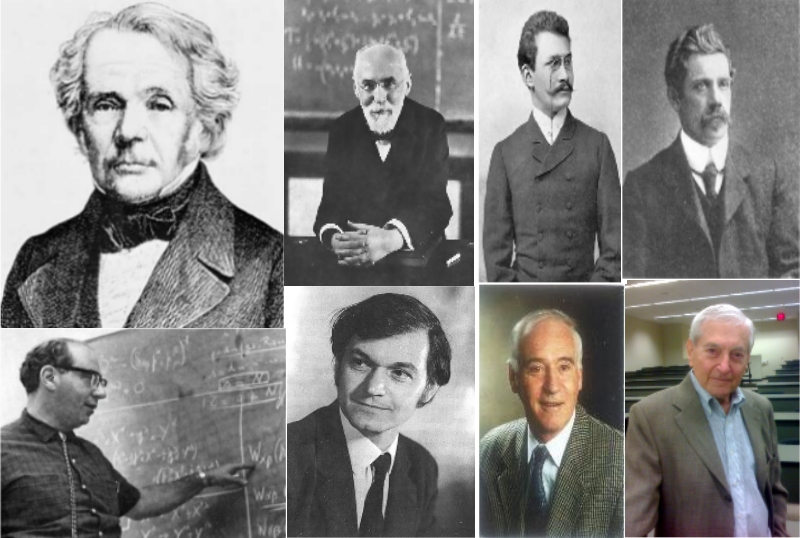
\includegraphics[scale=0.8]{figs/Cover.jpg}
%\end{center}
%\caption{\textit{}}
%\label{}
%\end{figure}

\newpage

\tableofcontents

\newpage

\pagenumbering{arabic}

\section{The Lorentz Transformation}

In this section the two null directions inherent in all Lorentz transformations, except the singular Lorentz transformations, are illustrated. The Lorentz Transform is defined by $(x,y,z,t) \rightarrow (x',y',z',t')$ such that

\begin{equation*}
{x'}^2 + {y'}^2 + {z'}^2 - {t'}^2 = x^2 + y^2 + z^2 - t^2.
\end{equation*}

\noindent If the transformation preserves the orientation of the spatial axes then is it called a \textit{proper} Lorentz transformation. This is equivalent to saying the transformation does not change the handedness of the axes. Also if $t \geq 0$ implies that time is always positive then it is called an \textit{orthochronous} Lorentz transformation, which ensures that the time direction is preserved. In this project the ``Lorentz transformation'' will refer to the proper, orthochronous Lorentz transformation.

Consider a photon moving in the $x$ direction at the speed of light, $c = 1$, and starting at $x = 0$. The space-time for such a photon can be illustrated as in Fig.() (FIGURE). It is clear that there are two null directions in this space-time, $x = \pm t$. To see this use the standard Lorentz transformation

\begin{align*}
x'  = \gamma (x - vt),  \\
t'  = \gamma (t - vx),
\end{align*}

\noindent where $\gamma = {(1 - v^2)}^{-1/2}$. Rearrange to obtain

\begin{eqnarray*}
x' - t' = \gamma (1 + v) (x - t), \\
x' + t' = \gamma (1 - v) (x + t).
\end{eqnarray*}

\noindent It is clear that $x = \pm t$ implies $x' = \pm t'$. Thus there are two null directions in this space-time at $x = \pm t$, as null directions are by definition invariant under a Lorentz transformation. It can be shown that all Lorentz transformations have two invariant null directions except the singular Lorentz transformation which has only one fixed null direction.  


\section{Reparameterisation of the Schwarzschild Solution}

In this section the Kasner solution of the vacuum field equations is derived from the Schwarzschild solution by taking the limit as the mass goes to infinity. It is then shown that the special case of the Kasner solution with no mass is equivalent to a novel form of Minkowskian space-time. Start with the Schwarzschild Solution of the vacuum field equations given by

\begin{equation}\label{Schwarz_Sol} 
\epsilon {\mathrm{d}s}^2 = {\left(1 - \frac{2m}{r}\right)}^{-1} {\mathrm{d}r}^{2} + r^2 ({\mathrm{d}\theta}^2 + {{\sin}^2 \theta}{\mathrm{d} \phi}^2) - \left(1 - \frac{2m}{r}\right) {\mathrm{d}t}^2.
\end{equation}

\subsection{Eddington-Finkelstein Coordinate Transformation}\label{Ed_Finkel_section}

\noindent First, make the Eddington-Finkelstein coordinate transformation

\begin{equation}\label{Ed-Fin_trans}
u = t - r - 2m \ln(r - 2m).
\end{equation}

\noindent This is generally used for a Schwarzschild geometry, particularly black holes. It is useful as it removes the singularity at the origin \cite{Finkelstein_Paper}. Calculate the differentials

\begin{align*}
\mathrm{d}u & = \mathrm{d}t - \mathrm{d}r - \frac{2m \mathrm{d}r}{r - 2m},\\
            & = \mathrm{d}t - \mathrm{d}r{\left( 1-\frac{2m}{r}  \right)}^{-1},\\
\mathrm{d}t & = \mathrm{d}u + {\left( 1-\frac{2m}{r}  \right)}^{-1} \mathrm{d}r, 
\end{align*}

\noindent and sub them into Eqn.(\ref{Schwarz_Sol}).

\begin{equation*}
\epsilon {\mathrm{d}s}^{2} = {\left( 1-\frac{2m}{r}  \right)}^{-1} \mathrm{d}r^2 + r^2 ({\mathrm{d}\theta}^2 + {{\sin}^2 \theta}{\mathrm{d} \phi}^2) - {\left( 1-\frac{2m}{r}  \right)} {\left( \mathrm{d}u + {\left( 1-\frac{2m}{r}  \right)}^{-1} \mathrm{d}r \right)}^{2},
\end{equation*}

\noindent which gives the result,

\begin{equation}\label{Reparameterisation_Schwarzschild_Before_Limit}
\epsilon {\mathrm{d}s}^{2} = r^2 ({\mathrm{d}\theta}^2 + {{\sin}^2 \theta}{\mathrm{d} \phi}^2) - 2 \mathrm{d}u \mathrm{d}r - {\mathrm{d}u}^{2} + \frac{2m}{r} {\mathrm{d}u}^{2}. 
\end{equation}

Note that if $m = 0$ the space-time becomes Minkowskian, as expected. If $r = 0$ in this Minkowskian space-time the line element becomes

$$ \epsilon {\mathrm{d}s}^2 = - {\mathrm{d}u}^{2},$$

\noindent which implies that $\epsilon = -1$ and the first integral of this trajectory is also equal to $-1$. Thus $r = 0$ is a time-like world-line in Minkowskian space-time, with proper time u. It can also be shown that $r=0$ is a geodesic with proper time, $u$ an affine parameter along it, this is done here in two ways. The first method is to write the line element in Cartesian coordinates using the transformation

\begin{gather*} 
x = r\sin{\theta}\cos{\phi}, \\
y = r\sin{\theta}\sin{\phi}, \\
z = r\cos{\theta}, \\
t = u + r.
\end{gather*}

\noindent It is clear that setting $r=0$ will give $x = y = z = 0$ and $t = u$. So the world-line is the t-axis with $u$ a parameter along it and is of course a time-like geodesic. The second method is much longer and involves calculating the metric and proving the geodesic equations, it is done here as it will be familiar to many readers. The Lagrangian method described by the following equations is used

\begin{gather*}
L = g_{ij} \dot{x}^{i}\dot{x}^{j},\\
\frac{d}{ds}\left( \frac{\partial L}{\partial \dot{x}^{i}}\right) - \frac{\partial L}{\partial {x}^{i}} = 2 w_{i}, \\
w^{j} = g^{ji}w_{i},  
\end{gather*}

\noindent with a geodesic defined by $w^{j} = 0$. The metric of this space-time in coordinates $(r ,\theta, \phi, u)$ is determined from Eqn.(\ref{Reparameterisation_Schwarzschild_Before_Limit}) with $m=0$

\begin{equation*}
g_{ij} = 
\left(
\begin{array}{cccc}
0  & 0 & 0             & -1 \\
0  & r & 0             & 0  \\
0  & 0 & r\sin{\theta} & 0  \\
-1 & 0 & 0             & -1 \\
\end{array}
\right).
\end{equation*}

\noindent The inverse of the metric is calculated to be

\begin{equation*}
g^{ij} =
\left(
\begin{array}{cccc}
1  & 0           & 0                       & -1 \\
0  & \frac{1}{r} & 0                       & 0  \\
0  & 0           & \frac{1}{r\sin{\theta}} & 0  \\
-1 & 0           & 0                       & 0  \\
\end{array}
\right).
\end{equation*}

\noindent $w^{j}$ will be calculated for $r$ and $u$ and simply stated for $\theta$ and $\phi$. The Lagrangian for $r$ is

\begin{equation*}
w_{r} = - \ddot{u} - r (\dot{\theta}^2 + \sin^2{\theta}\dot{\phi}^2),
\end{equation*}

\noindent and the Lagrangian for $u$ is

\begin{equation*}
w_{u} = - \ddot{u} - \ddot{r}  
\end{equation*}
 
\noindent Now $w^{r}$ is given by

\begin{align*}
w^{r} & = g^{rj} w_{j} \\
      & = w_{r} - w_{u}
\end{align*}

\noindent and $w^{u}$ is

\begin{align*}
w^{u} & = g^{uj} w_{j} \\
      & =  - w_{r}
\end{align*}

\noindent So putting these together to obtain $w^{r} = 2w_{r}$ and $w^{u} = -w_{r}$ which implies

\begin{align*}
w^{r} & = -2 \ddot{u} - 2 r(\dot{\theta}^2 + \sin^2{\theta}\dot{\phi}^2), \\
w^{u} & = \ddot{u} + r(\dot{\theta}^2 + \sin^2{\theta}\dot{\phi}^2), \\
\end{align*}

\noindent and also for $\theta$ and $\phi$

\begin{align*}
w^{\theta} = r \ddot{\theta} + 2 \dot{\theta} \dot{r} - r \sin{\theta}\cos{\theta}\dot{\phi}^2, \\
w^{\phi} = \sin{\theta}(\dot{\phi} \dot{r} + r \ddot{\phi}) + 2r \dot{\phi}\cos{\theta} \dot{\theta}.
\end{align*}

\noindent Then set $r=0$ to obtain the equations

\begin{align*} 
w^{r} = - 2 \ddot{u}, \\
w^{u} = \ddot{u}, \\
w^{\theta} = 0, \\
w^{\phi} = 0,.
\end{align*} 

\noindent Now $s = u$ as $u$ is proper time then $w^{r} = w^{u} = 0$, which implies that the trajectory $r=0$ is a geodesic with $u$ an affine parameter along it. 

The limit of the Schwarzschild solution as $m \rightarrow \infty$ must be calculated to find the Kasner solution. In its current form the limit cannot be taken, so two suitable coordinate transformations must be made to get it in a more useful form. First Set 

\begin{gather*} 
u = \mu u', \\
r = {\mu}^{-1} r',   
\end{gather*} 

\noindent where $\mu = \text{ const}$ so that
  
\begin{gather*} 
\mathrm{d}u = \mu \mathrm{d}u', \\
\mathrm{d}r = {\mu}^{-1} \mathrm{d}r'. \\
\end{gather*} 

\noindent The product of the differentials is then invariant

\begin{equation*}
{\mathrm{d}u}{\mathrm{d}r} = {\mathrm{d}u'}{\mathrm{d}r'}. 
\end{equation*}

\noindent When the new coordinates are subbed into Eqn.(\ref{Reparameterisation_Schwarzschild_Before_Limit}) the Schwarzschild solution becomes

\begin{equation}\label{Reparameterise_Schwarzschild_Next_Before_Limit}
\epsilon {\mathrm{d}s}^2 = {r'}^2 \sin^2 \theta \left\{ \frac{{\mathrm{d}\theta}^2}{\mu^2 \sin^2 \theta} +  \mu^{-2} {\mathrm{d} \phi}^2 \right\} - 2 {\mathrm{d}u'} {\mathrm{d}r'} - \left( \mu^2 - \frac{2 m \mu^3}{r'}\right) {\mathrm{d}u'}^2 . 
\end{equation}

\noindent Now set $m \mu^{3} = k$ or $ m = k \mu^{-3}$ and make another transformation first done by Ivor Robinson given by \cite{I_Robinson_Paper}

\begin{align*} 
\sin{\theta} = \frac{1}{\cosh{(\mu \xi)}}, \qquad  \mu^{-1} \phi = \eta.  
\end{align*} 

\noindent The second of these transformations gives simply $\mu^{-2} \mathrm{d}\phi^2 = \mathrm{d} \eta^2$. To rewrite the first coordinate transformation, first differentiate.

\begin{align*} 
\cos{\theta} \mathrm{d} \theta & = \frac{-1}{(\cosh(\mu \xi))^{2}} \sinh(\mu \xi) \mu \mathrm{d} \xi, \\
                      & = -{\sin}^{2}\theta \sinh(\mu \xi) \mu \mathrm{d} \xi.
\end{align*}

\noindent Use the formula $\cosh^2 A - \sinh^2 A = 1$, divide by $\mathrm{d} \xi$ and simplify using trigonometric identities

\begin{align*}
\cos{\theta} \frac{\mathrm{d} \theta}{\mathrm{d} \xi} & = -\mu \sin^2 \theta \sqrt{\frac{1}{\sin^2 \theta} - 1}, \\
                                    & = - \mu \sin \theta \cos \theta.
\end{align*}

\noindent Finally rewrite in terms of $\mathrm{d} \xi$

\begin{equation*}
\mathrm{d} \xi^2 = {\left( \frac{\mathrm{d} \theta}{\mu \sin \theta}  \right)}^2.
\end{equation*}

\noindent Subbing these transformations into Eqn.(\ref{Reparameterise_Schwarzschild_Next_Before_Limit}) gives

\begin{equation*}
\epsilon {\mathrm{d}s}^2 = \frac{r^2}{\cosh^{2}{\mu \xi}} ({\mathrm{d}\xi}^2 + {\mathrm{d}\eta}^2) - 2 {\mathrm{d}u}{\mathrm{d}r} - \left( \mu^{2} - \frac{2k}{r} \right) {\mathrm{d}u}^2,
\end{equation*}

\noindent where the primes have been dropped for convenience. 

\subsection{The Kasner Solution}

This is now in an appropriate form to take the limit $m \rightarrow \infty$ which is equivalent to $\mu \rightarrow 0$, to obtain

\begin{equation}\label{Kasner_after_limit}
\epsilon {\mathrm{d}s}^2 = r^2 ({\mathrm{d}\xi}^2 + {\mathrm{d}\eta}^2) - 2 {\mathrm{d}u}{\mathrm{d}r} - \frac{2k}{r} {\mathrm{d}u}^2
\end{equation}

\noindent This is still a solution of the field equations but it is no longer the Schwarzschild solution. In this section it is shown to be the Kasner Solution, which by definition is given by

\begin{equation}\label{Reparameterise_Definition_Of_Kasner} 
\epsilon {\mathrm{d}s}^2 = T^{2p} {\mathrm{d}X}^2 + T^{2q} \mathrm{d}Y^2 + T^{2r} \mathrm{d}Z^2 - \mathrm{d}T^2,
\end{equation}

\noindent such that

\begin{eqnarray*}
p + q + r = 1 = p^2 + q^2 + r^2.
\end{eqnarray*}

This solution is characteristic of aniosotropic space-times, which means it is directionally dependant. To write Eqn.(\ref{Kasner_after_limit}) in the above form first make the transformation

\begin{gather*} 
\xi' = \lambda^{-1} \xi, \text{    }  \eta' = \lambda^{-1} \eta, \\
r' = \lambda r,          \text{    }  u' = \lambda^{-1} u,
\end{gather*}

\noindent with $\lambda \vcentcolon = k^{-1/3}$. Subbing in these new coordinates gives

\begin{equation*}  
\epsilon \mathrm{d} s^2 = {r'}^2 (\mathrm{d} {\xi'}^2 + \mathrm{d} {\eta'}^2) - 2 \mathrm{d} u' \mathrm{d} r' + \frac{2}{r'}\mathrm{d} {u'}^2.
\end{equation*}

\noindent Now add and subtract $(r'/2) \mathrm{d} {r'}^2$ to complete the square as follows

\begin{equation*}  
\epsilon \mathrm{d} s^2 = r^2 (\mathrm{d} \xi^2 + \mathrm{d} \eta^2) + \frac{2}{r}{\left( \mathrm{d} u  - \frac{r}{2} \mathrm{d} r\right)}^2 - \frac{r}{2}\mathrm{d} r^2,
\end{equation*}

\noindent where the primes have again been dropped for convenience. Now set

\begin{equation*}
\bar{X} = u - \frac{r^2}{4},
\end{equation*}

\noindent so the differential of $\bar{X}$ is

\begin{equation*}
\mathrm{d} \bar{X} = \mathrm{d} u - \frac{r}{2} \mathrm{d}r,
\end{equation*}

\noindent and the line element can be rewritten in terms of $\bar{X}$,

\begin{equation*}
\epsilon \mathrm{d} s^2 = r^2 (\mathrm{d} \xi^2 + \mathrm{d} \eta^2) + \frac{2}{r} \mathrm{d} \bar{X}^2 - {\left( \frac{r^{1/2}}{\sqrt{2}} \mathrm{d} r\right)}^{2}.
\end{equation*}

\noindent Now define $T$ such that

\begin{equation*}
T = \frac{\sqrt{2}}{3} r^{3/2} \text{,       and    } r = {\left( \frac{3}{\sqrt{2}} \right)}^{2/3} T^{2/3},
\end{equation*}

\noindent which results in the new line element

\begin{equation*}
\epsilon \mathrm{d} s^2 = \left( \frac{3}{\sqrt{2}} \right)^{4/3} T^{4/3} (\mathrm{d} \xi^2 + \mathrm{d} \eta^2) + 2 \left( \frac{\sqrt{2}}{3}\right)^{2/3} T^{-2/3} \mathrm{d} \bar{X}^2 - \mathrm{d} T^2.
\end{equation*}

\noindent Then a final coordinate transformation can be made to remove the unwanted constants, given by

\begin{align*} 
X & = \left[ 2\left( \frac{\sqrt{2}}{3}\right)\right]^{1/2} \bar{X}, \\
Y & = \left( \frac{3}{\sqrt{2}} \right)^{2/3} \xi, \\
Z & = \left( \frac{3}{\sqrt{2}} \right)^{2/3} \eta, \\
\end{align*} 

\noindent to obtain

\begin{equation}\label{Our_Kasner} 
\epsilon {\mathrm{d}s}^2 = T^{-2/3} {\mathrm{d}X}^2 + T^{4/3} \left( \mathrm{d}Y^2 + \mathrm{d}Z^2 \right) - \mathrm{d}T^2.
\end{equation}

\noindent Comparing this result to the general form of the Kasner solution in Eqn.(\ref{Reparameterise_Definition_Of_Kasner}) it is clear that they have the same form with $p=-1/3$ and $q=r=2/3$. Thus the solution obtained by taking the limit of the Schwarzschild solution as $m \rightarrow \infty$ is indeed the Kasner Solution. 

\subsection{Line Element of Minkowskian Space-Time}

Minkowskian space-time reemerges again by setting the energy, $k = 0$ in Eqn.(\ref{Kasner_after_limit}), which is equivalent to $m = 0$. 

\begin{equation}\label{Kasner_after_limit_no_k}
\epsilon {\mathrm{d}s}^2 = r^2 ({\mathrm{d}\xi}^2 + {\mathrm{d}\eta}^2) - 2 {\mathrm{d}u}{\mathrm{d}r}
\end{equation}

\noindent Setting $r = 0$ gives $\epsilon {\mathrm{d}s}^2 = 0$. In this section it is demonstrated that $r = 0$ is a null geodesic with $u$ an affine parameter along it and that Eqn.(\ref{Kasner_after_limit_no_k}) is indeed the Minkowskian space-time line element. To verify these properties first let $x^i = (x,y,z,t)$ be rectangular Cartesian coordinates with time in Minkowskian space-time with the usual line element

\begin{equation*} 
\epsilon {\mathrm{d}s_0}^2 = {\mathrm{d}x}^2 + {\mathrm{d}y}^2 + {\mathrm{d}z}^2 - {\mathrm{d}t}^2.
\end{equation*} 

\noindent We note that the trajectory $C$  defined by $x = 0$, $y = 0$, $z = t$ is a null geodesic as it will lie on the light cone of Minkowskian space-time. 

\begin{figure}[h!]
\begin{center}
\caption{\textit{Minkowskian space-time illustrating the new parameter $r$ which is the shortest distance between some point $x^i$ and the trajectory $C$ along the $k^i$ direction. The parameter $u$ which determines the distance travelled along $C$ is also shown}}
\label{Reparameterization_Figure_Unit_Vector}
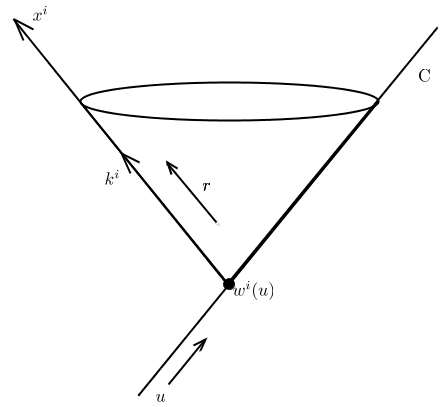
\includegraphics[scale=0.8]{figs/2_1.png}
\end{center}
\end{figure}

\noindent If $C$ is written parametrically as $x^i = w^i (u)$ such that $w^i = (0,0,u,u)$ then $u$ is an affine parameter along it. The tangent to $C$ is then computed as

\begin{equation*} 
v^i (u) = \frac{\mathrm{d} w^i}{\mathrm{d}u} = (0,0,1,1).
\end{equation*} 

\noindent As $C$ is a null geodesic the first integral will be $v_i v^i = 0$ and thus $v_i = (0,0,1,-1)$ where we have chosen the convention $(+,+,+,-)$. The position vector of a point in Minkowskian space time can be written in the form

\begin{eqnarray*}
x^i - w^i (u) = r k^i, \\
\text{or } x^i = w^i(u) + r k^i. 
\end{eqnarray*}

\noindent Thus $r$ is a new parameter which gives the shortest distance between $C$ and some point $x^i$, and $k^i$ is the unit vector in that direction, see Fig.(\ref{Reparameterization_Figure_Unit_Vector}). As $k^i$ is a unit vector it satisfies the relations

\begin{gather}
k^i k_i = 0 \label{k_rel_1},\\
k^i v_i = -1 \label{k_rel_2}.
\end{gather}

\noindent Thus $k^i$ is normalized so that $k^i$ and $v^i$ are both future pointing. Making the parameterisation

\begin{gather*}
k^i = (\xi, \eta, A, B), \\
k_i = (\xi, \eta, A, -B).
\end{gather*}

\noindent We can choose any variable for the first two slots of $k^i$ so we choose $\xi$ and $\eta$ from before for convenience. Using the relation (\ref{k_rel_1}) it is clear that

\begin{equation*}
\xi^2 + \eta^2 + A^2 - B^2 = 0,
\end{equation*}

\noindent and using the relation (\ref{k_rel_2}) it is found that

\begin{gather}
A - B = -1 \label{sim_rel_1},\\
A^2 - B^2 = (A + B)(A - B) = - (A + B).
\end{gather}

\noindent Which implies

\begin{equation}\label{sim_rel_2}
\xi^2 + \eta^2 = A + B. 
\end{equation}

\noindent So expressions for $A$ and $B$ are found using Eqn.(\ref{sim_rel_1}) and Eqn.(\ref{sim_rel_2}):

\begin{eqnarray*}
A = \frac{1}{2} (-1 + \xi^2 + \eta^2) \\
B = \frac{1}{2} (1 + \xi^2 + \eta^2) \\
\end{eqnarray*}

In summary so far we have

\begin{align}
x^i & = w^i (u) + r k^i \label{rel_for_trans_1},\\
w^i & = (0,0, u,u) \label{rel_for_trans_2},\\
k^i & = (\xi, \eta, \frac{1}{2} (-1 + \xi^2 + \eta^2), \frac{1}{2} (1 + \xi^2 + \eta^2)) \label{rel_for_trans_3},\\
x^i & = (x, y, z, t) \label{rel_for_trans_4}.  
\end{align}

Consider Eqn.(\ref{rel_for_trans_1}) as a coordinate transformation from $(x,y,z,t)$ to $(\xi,\eta, r, u )$ such that

\begin{align}
x & = r \xi, \nonumber \\
y & = r \eta, \nonumber \\
z & = u + \frac{r}{2} (-1 + \xi^2 + \eta^2), \nonumber \\
t & = u + \frac{r}{2} (1 + \xi^2 + \eta^2),  \label{trans_x_to_xi} 
\end{align} 

\noindent which is clear from Eqns.(\ref{rel_for_trans_1}) - (\ref{rel_for_trans_4}). Now this is applied to the Minkowskian line element of Eqn.(\ref{Kasner_after_limit_no_k}). First, the $x$ and $y$ differentials are

\begin{eqnarray*} 
dx = r \mathrm{d}\xi + \xi \mathrm{d}r, \\
\mathrm{d}y = r \mathrm{d}\eta + \eta \mathrm{d}r. 
\end{eqnarray*} 

\noindent Which gives

\begin{equation}\label{differentials_1}
{\mathrm{d}x}^2 + {\mathrm{d}y}^2 = r^2 ({\mathrm{d}\xi}^2 + {\mathrm{d}\eta}^2) + 2 r \xi {\mathrm{d}\xi} {\mathrm{d}r} + 2 r \eta {\mathrm{d}\eta}{\mathrm{d}r} + (\xi^2 + \eta^2) {\mathrm{d}r}^2.
\end{equation}

\noindent Next, the $z$ and $t$ differentials

\begin{align*}
z + t & = 2 u + r (\xi^2 + \eta^2), \\
z - t & = - r, \\
{\mathrm{d}z} + {\mathrm{d}t} & = 2 \mathrm{d}u + (\xi^2 + \eta^2) \mathrm{d}r + 2 r \xi {\mathrm{d}\xi} + 2 r \eta {\mathrm{d}\eta}, \\
{\mathrm{d}z} - {\mathrm{d}t} & = - \mathrm{d}r. 
\end{align*}

\noindent Then using difference of two squares to obtain

\begin{equation}\label{differentials_2}
{\mathrm{d}z}^2 - {\mathrm{d}t}^2 = -2 {\mathrm{d}u}{\mathrm{d}r} - (\xi^2 + \eta^2) {\mathrm{d}r}^2 - 2 r \xi {\mathrm{d}\xi}{\mathrm{d}r} - 2 r \eta {\mathrm{d}\eta}{\mathrm{d}r}.
\end{equation}

\noindent Combining Eqn.(\ref{differentials_1}) and (\ref{differentials_2}) to get:

\begin{equation*}
{\mathrm{d}x}^2 + {\mathrm{d}y}^2 + {\mathrm{d}z}^2 - {\mathrm{d}t}^2 = r^2 ({\mathrm{d}\xi}^2 + {\mathrm{d}\eta}^2) - 2 {\mathrm{d}u}{\mathrm{d}r}
\end{equation*}

\noindent and from this it is clear that Eqn.(\ref{Kasner_after_limit_no_k}) is the line element of Minkowskian space-time with $r = 0$ a null geodesic with affine parameter $u$ along it as stated in Section (\ref{Ed_Finkel_section}).

Thus it has been shown that the Kasner solution to the vacuum filed equations can be obtained from the Schwarzschild solution of the vacuum field equations by taking the special case where the mass goes to infinity. Then the Minkowskian space-time line element in a particular set of coordinates $(\xi, \eta, r, u)$, can be derived from the Kasner solution by setting the energy, $k$ to zero. It has been shown that the special case where $r=0$ in this Minkowskian space-time is then a null geodesic with $u$ an affine parameter along it.  


\section{The Singular Lorentz Transformation}

In this section a Lorentz transformation that leaves our line element Eqn.(\ref{Kasner_after_limit_no_k}) invariant is constructed. This transformation is then expressed in terms of $(x,y,z,t)$ and examined to see what form it has. The subgroup of the Lorentz group that it makes is then examined. First define an arbitrary complex parameter by $\zeta = \xi + i \eta$ so that the differentials are given by \cite{Hogan}

\begin{eqnarray*}
d\zeta = {d\xi} + i {d\eta}, \\
d\bar{\zeta} = {d\bar{\xi}} - i {d\bar{\eta}}, \\
\end{eqnarray*}

\noindent and the line element can be rewritten as

\begin{equation*}
\epsilon {ds^2} = r^2 {d\zeta}{d\bar{\zeta}} - 2 {du}{dr}.
\end{equation*}

\noindent In this form the transformation $\zeta \rightarrow \zeta + w$, where $w \in \mathbb{C}$, is trivial. It leaves the line element unchanged and the null geodesic $r = 0$ trivially invariant. This is a Lorentz transformation which leaves one null direction invariant. Therefore it is a two real parameter, singular Lorentz transformation, where the two parameters come from the complex variable $w$. With this form of the line element the transformation is obviously trivially invariant. What does this transformation look like in terms of the usual coordinates $(x,y,z,t)$?

First invert the transformation (\ref{trans_x_to_xi}) and use the new variable $\zeta$

\begin{align} \nonumber
x + iy  & = r (\xi + i \eta) = r \zeta \\\nonumber
z  & = u + \frac{r}{2}(-1 + \zeta \bar{\zeta}) \\\label{Singular_Trans_x,y,z,t_xi,eta,r,u_first}
t &  = u + \frac{r}{2}(1 + \zeta \bar{\zeta})
\end{align}

\noindent From this it is clear that

\begin{align*}
t - z & = r, \\
t + z & = 2 u + r \zeta \bar{\zeta}. 
\end{align*}

\noindent So finally

\begin{align}\nonumber
r & = t - z, \\\nonumber
\zeta & = \frac{x + i y}{t-z}, \\\label{Singular_Trans_x,y,z,t_xi,eta,r,u_second}
u & = \frac{1}{2} (t + z) - \frac{(x^2 + y^2)}{2(t - z)}.
\end{align}

\noindent Now make the desired transformation $(\zeta', \bar{\zeta}', r', u') \rightarrow (\zeta + w, \bar{\zeta} + \bar{w}, r, u)$ by first replacing these new quantities into transformation (\ref{Singular_Trans_x,y,z,t_xi,eta,r,u_first})

\begin{align*}
x' + iy' & = r'\zeta' = r(\zeta + w), \\
z' & = u + \frac{r}{2}(-1 + \zeta \bar{\zeta} + \zeta \bar{w} + \bar{\zeta} w + w \bar{w}), \\
t' & = u + \frac{r}{2} (1 + \zeta \bar{\zeta} + \zeta \bar{w} + \bar{\zeta} w + w \bar{w}). 
\end{align*}

\noindent So the transformed Cartesian coordinates have been written in terms of the untransformed particular coordinates, $(\zeta, r, u)$. Next, using the relations (\ref{Singular_Trans_x,y,z,t_xi,eta,r,u_second}), write the transformed Cartesian coordinates in terms of the untransformed Cartesian coordinates.

\begin{align}
x' + i y' & = x + iy + w(t-z) \label{sing_final_no_prime_1}, \\
z' - t' & = -r = z - t \label{sing_final_no_prime_2}, \\
z' + t' & = z+t + w(x - i y) + w(x + iy) + w\bar{w} (t-z) \label{sing_final_no_prime_3}.
\end{align}

It is necessary to show that this is indeed a Lorentz transformation by verifying the usual Lorentz invariant quadratic form. First, Eqn.(\ref{sing_final_no_prime_1}) implies

\begin{align*}
{x'}^2 + {y'}^2 &  = (x + iy + w(t-z))(x - iy + \bar{w}(t-z)) \\
& = x^2 + y^2 + \bar{w}(t - z)(x+iy) + w(t-z)(x-iy) + w\bar{w}{(t-z)}^2.
\end{align*}

\noindent Then Eqn.(\ref{sing_final_no_prime_2}) and Eqn.(\ref{sing_final_no_prime_3}) imply

\begin{align*}
{z'}^2 - {t'}^2 & = (z' + t')(z' - t') \\
& = z^2 - t^2 + (z - t)w(x-iy) + (z-t)\bar{w}(x+iy) + (z -t)w\bar{w}(t-z)
\end{align*}

\noindent Thus the extra terms cancel and the Lorentz invariant quadratic form in the primed frame is the same as that of the unprimed frame,

\begin{equation*} 
{x'}^2 + {y'}^2 + {z'}^2 - {t'}^2 = {x}^2 + {y}^2 + {z}^2 - {t}^2.
\end{equation*} 

\noindent It is also clear from Eqn.(\ref{sing_final_no_prime_2}) that the null direction $z = t$ is invariant under this Lorentz transformation.

In conclusion, this transformation involves one complex parameter, $w$ and thus two real parameters. In the usual Cartesian coordinates it is described by Eqns.(\ref{sing_final_no_prime_1}) - (\ref{sing_final_no_prime_3}) and in the coordinates $(\xi, \eta, r, u)$, also denoted by $(\zeta, r,u)$ derived in previous sections, it is expressed simply as

\begin{align*}
\zeta' & = \zeta + w, \\
r' & = r, \\
u' & = u.
\end{align*}

Note that the operation of addition of complex numbers is commutative so that if $\zeta' = \zeta + w_1$ and $\zeta'' = \zeta' + w_2$ then

\begin{equation*} 
\zeta'' = \zeta + w_1 + w_2 = \zeta + w_3.
\end{equation*} 
 
\noindent Thus these transformations form a 2-parameter abelian subgroup of the Lorentz group with the binary operation of addition of complex numbers.

So a Lorentz transformation that preserves the line element Eqn.(\ref{Kasner_after_limit_no_k}) has been constructed. It is found that this transformation is a singular Lorentz transformation as it keeps the null direction $r=0$ fixed. Thus it is shown that \textit{all singular Lorentz transformations are two parameter abelian subgroups of the Lorentz group}. Note that not all two parameter abelian subgroups of the Lorentz group are singular Lorentz transformations.  








\section{Special Linear Matrices of the Lorentz Transformation}\label{Special_Linear_Matrices_of_Lorentz}

In this section it is shown that there is a $2$ to $1$ correspondence between the matrices $SL(2, \mathbb{C})$ and the proper orthochronous Lorentz transformations. First it is demonstrated that there is a one to one correspondence between $2 \times 2$ Hermitian matrices and Minkowskian space-time, this is then applied to Lorentz transformations. Let $\vec{x} = (x,y,z,t)$ be the position vector of a point in Minkowskian space-time. Knowing $\vec{x}$ we can construct the following $2 \times 2$ Hermitian matrix \cite[p. 9-10]{Hypersurfaces_Hogan_Barrabes}

\begin{equation}\label{Special_Matrices_A_first}
A = 
\left( 
\begin{array}{cc}
t-z    & x + i y \\
x - iy & t+z \\
\end{array} 
\right),
\end{equation}

\noindent with $A^{\dagger}(\vec{x}) = A(\vec{x})$. This is useful as its determinant is the same as the Lorentz invariant quadratic form, up to an arbitrary sign.

\begin{equation*}
\det(A(\vec{x})) = t^2 - x^2 - y^2 - z^2.
\end{equation*}

\noindent This form also has a connection to spinors (ERROR. check formula, Lie Algebras? look at RQM notes, reference to spinor scetion if i write one, pg2 references) 

\begin{equation*}
A = [t\mathcal{I}_{2} - \vec{x} \cdot \vec{\sigma}]
\end{equation*}  

Consider any $2 \times 2$ Hermitian matrix $H$, thus

\begin{equation*}
H = \left( \begin{array}{cc}
p & q \\
r & s \\
\end{array} \right) \text{ ,     }
H^{\dagger} = \left( \begin{array}{cc}
\bar{p} & \bar{r} \\
\bar{q} & \bar{s} \\
\end{array} \right)
\end{equation*}

\noindent It is know that $H^{\dagger}(\vec{x}) = H(\vec{x})$ so it is clear that $p = \bar{p}$ and $s = \bar{s}$ and thus $p$ and $s$ are real numbers. Also $q = \bar{r}$ and then of course $\bar{q} = r$. Hence knowing $p,q,r$ and $s$ is equivalent to knowing $4$ real numbers, one from $p$, one from $s$ and two from $q$. From these parameters the coordinates $(x,y,z,t)$ of a point in Minkowskian space-time can be constructed as

\begin{align*}
x + iy & = q = \bar{r}, \\
t - z & = p, \\
t+z  & = s.
\end{align*}

\noindent by comparing with matrix $A$ above. Hence it is true that there is a one to one correspondence between points in Minkowskian space-time and $2 \times 2$ Hermitian matrices.

Construct the following matrix

\begin{equation*} 
U = \left( 
\begin{array}{cc}
\alpha & \beta \\
\gamma & \delta \\
\end{array}
\right),
\end{equation*}

\noindent with $\alpha$, $\beta$, $\gamma$, $\delta \in \mathbb{C}$, and the condition that $\det(U) = 1$. Such matrices $U$ form a group called the special linear group, which is denoted by $SL(2, \mathbb{C})$. Given $A(\vec{x})$ consider $U A(\vec{x}) U^{\dagger}$. This is a $2 \times 2$ Hermitian matrix since

\begin{align*}
(U A(\vec{x}) U^{\dagger})^{\dagger} & =  (U^{\dagger})^{\dagger} A^{\dagger}(\vec{x}) U^{\dagger} \\
                                     & = U A(\vec{x}) U^{\dagger},
\end{align*} 

\noindent as $(U^{\dagger})^{\dagger} = U$ and $A^{\dagger} = A$. Hence there exists a point $\vec{x}' = (x', y', z', t')$ in Minkowskian space-time for which

\begin{equation}\label{SL_trans}
A(\vec{x}') = U A(\vec{x}) U^{\dagger}.
\end{equation}

Any $U$ involves 6 real parameters, 2 each from the four complex components, with the condition $\det(U) = 1$ supplying two constraints, one on the real parts and one on the imaginary parts of the components. Now calculate the determinant of the matrix in the primed frame

\begin{align*}  
\det(A(\vec{x}')) & = \det(U A(\vec{x}) U^{\dagger}), \\
                  & = (\det(U))(\det(A(\vec{x}))(\det(U^{\dagger})), \\
                  & = (\det(U))(\det(A(\vec{x}))\bar{(\det(U))}, \\
                  & = \det(A(\vec{x})).
\end{align*}

\noindent Thus we have the relation

\begin{equation*}  
{t'}^2 - {x'}^2 - {y'}^2 - {z'}^2 = {t}^2 - {x}^2 - {y}^2 - {z}^2.
\end{equation*}

\noindent Hence the transformation $\vec{x} \rightarrow \vec{x}'$ implicit in Eqn.(\ref{SL_trans}) is a Lorentz transformation. This equation describes the most general proper, orthochronous Lorentz transformation.

It is useful to calculate the matrix $U$ for some examples of Lorentz transformations. First, write Eqn.(\ref{SL_trans}) in terms of its components

\begin{align*} 
\left(
\begin{array}{cc}
t' - z' & x' + i y' \\
x' - i y' & t' + z' \\
\end{array}
\right)
& =
\left(
\begin{array}{cc}
\alpha & \beta \\
\gamma & \delta \\
\end{array}
\right)
\left(
\begin{array}{cc}
t-z & x + i y \\
x - i y & t + z   \\
\end{array}
\right)
\left(
\begin{array}{cc}
\bar{\alpha} & \bar{\gamma} \\
\bar{\beta} & \bar{\delta} \\
\end{array}
\right), \\
& = \left(
\begin{array}{cc}
\alpha & \beta \\
\gamma & \delta \\
\end{array}
\right)
\left(
\begin{array}{cc}
(t-z)\bar{\alpha} + (x + iy)\bar{\beta} & (t-z)\bar{\gamma} + (x + iy)\bar{\delta} \\
(x - iy)\bar{\alpha} + (t+z)\bar{\beta} & (x-iy)\bar{\gamma} + (t+z)\bar{\delta} \\
\end{array}
\right).
\end{align*}

\noindent Thus the relations

\begin{subequations}
\begin{gather}\label{general_coeff_equate_a}
t' - z'  = (t-z)\alpha\bar{\alpha} + (x + iy)\alpha\bar{\beta} + (x - iy)\beta\bar{alpha} + (t+z)\beta\bar{\beta},
\\\label{general_coeff_equate_b}
x' + iy'  = (t-z)\alpha\bar{\gamma} + (x + iy)\alpha\bar{\delta} + (x-iy)\beta\bar{\gamma} + (t+z)\beta\bar{\delta},
\\\label{general_coeff_equate_c}
t' + z'  = (t-z)\gamma\bar{\gamma} + (x + iy)\gamma\bar{\delta} + (x-iy)\delta\bar{\gamma} + (t+z)\delta\bar{\delta}.
\end{gather}
\end{subequations}

\noindent are obtained. Now these equations are used on some specific cases.

\subsection{Example 1: Rotational Transformation}

\noindent Find $U$ corresponding to the one parameter Lorentz transformation,

\begin{align*} 
x' & = x\cos{\theta} + y\sin{\theta}, \\
y' & = -x\sin{\theta} + y\cos{\theta}, \\
z' & = z, \\
t' & = t.
\end{align*} 

\noindent This implies that

\begin{align*}
t'-z' & = t-z \\
x'+iy' & = (x+iy) e^{-i \theta} \\
t'+z' & = t+z
\end{align*}

\noindent Equating coefficients of $x$, $y$, $z$, $t$ on both sides of Eqn.(\ref{general_coeff_equate_a}) to obtain

\begin{subequations}
\begin{gather}\label{Ex1_equate_coeffs_first_a}
\alpha \bar{\beta} + \bar{\alpha} \beta = 0, \\\label{Ex1_equate_coeffs_first_b}
i (\alpha \bar{\beta} - \bar{\alpha} \beta) = 0, \\\label{Ex1_equate_coeffs_first_c}
-\alpha \bar{\alpha} + \beta \bar{\beta} = -1, \\\label{Ex1_equate_coeffs_first_d}
\alpha \bar{\alpha} + \beta \bar{\beta} = 1. 
\end{gather}
\end{subequations}

\noindent Then Eqn.(\ref{Ex1_equate_coeffs_first_a}) and (\ref{Ex1_equate_coeffs_first_b}) imply $\alpha \bar{\beta} = 0$ so $\alpha = 0$ or $\beta = 0$. Also Eqn.(\ref{Ex1_equate_coeffs_first_c}) and (\ref{Ex1_equate_coeffs_first_d}) imply $2\beta\bar{\beta} = 0$ so $\beta = 0$ and $\alpha \bar{\alpha} = 1$ so $\alpha \neq 0$. Equating coefficients of $x$, $y$, $z$, $t$ on both sides of Eqn.(\ref{general_coeff_equate_b}) to obtain

\begin{subequations}
\begin{gather}\label{Ex1_equate_coeffs_second_a}
e^{-i\theta} = \alpha \bar{\delta} + \beta\bar{\gamma}, \\\label{Ex1_equate_coeffs_second_b}
e^{-i\theta} = \alpha \bar{\delta} - \beta\bar{\gamma},\\\label{Ex1_equate_coeffs_second_c}
0 = -\alpha\bar{\gamma} + \beta \bar{\delta},\\\label{Ex1_equate_coeffs_second_d}
0 = \alpha\bar{\gamma} + \beta \bar{\delta}. 
\end{gather}
\end{subequations}

\noindent With $\beta = 0$, Eqn.(\ref{Ex1_equate_coeffs_second_a}) and (\ref{Ex1_equate_coeffs_second_b}) imply $\alpha \bar{\delta} = e^{-i\theta}$. Also Eqn.(\ref{Ex1_equate_coeffs_second_c}) and (\ref{Ex1_equate_coeffs_second_d}) imply $\alpha \bar{\gamma} = 0$ so $\gamma = 0$ since $\alpha \neq 0$. Then using $\alpha \bar{\alpha} =1$

\begin{align*}
\alpha \bar{\delta} & = e^{-i\theta}, \\
\bar{\alpha} \alpha \bar{\delta} & = \bar{\alpha} e^{-i\theta},\\
\bar{\delta}  & =  \bar{\alpha} e^{-i\theta}.
\end{align*}

\noindent Equating coefficients of $x$, $y$, $z$, $t$ on both sides of Eqn.(\ref{general_coeff_equate_c}) to obtain

\begin{subequations}
\begin{gather}\label{Ex1_equate_coeffs_third_a}
\gamma \bar{\delta} + \delta \bar{\gamma} = 0, \\\label{Ex1_equate_coeffs_third_b}
\gamma \bar{\delta} - \delta \bar{\gamma} = 0 ,\\\label{Ex1_equate_coeffs_third_c}
-\gamma \bar{\gamma} + \delta \bar{\delta} = 1 ,\\\label{Ex1_equate_coeffs_third_d}
\gamma \bar{\gamma} + \delta \bar{\delta} = 1. 
\end{gather}
\end{subequations}

\noindent Eqn(\ref{Ex1_equate_coeffs_third_a}) and (\ref{Ex1_equate_coeffs_third_b}) are satisfied since $\gamma = 0$, this also implies that $\delta \bar{\delta} = 1$ from Eqn(\ref{Ex1_equate_coeffs_third_c}). Now use the fact that $\det{(U)} = 1$, which implies

\begin{equation*}
\alpha \delta - \beta \gamma = 1,
\end{equation*}

\noindent thus $\alpha \delta = 1$ as $\beta = 0$. Then using $\alpha \bar{\alpha} = 1$ again and $\delta \bar{\delta} = 1$

\begin{align*}
\alpha^2 e^{-\theta} & = 1, \\
\alpha^2 & = e^{-i\theta}, \\
\alpha & = \pm e^{{-i\theta}/2}, 
\end{align*}

\noindent which finally implies that $\delta = \pm e^{i\theta/2}$. Hence there are 2 matrices $U$ corresponding to the spacial rotation, namely

\begin{equation*}
U = \pm
\left(
\begin{array}{cc}
e^{-i\theta/2} & 0            \\
0              & e^{i\theta/2} \\
\end{array}
\right)
\end{equation*}

\noindent The next two examples are then very similar.

\subsection{Example 2: Standard Lorentz Transformation}\label{Special_Linear_Matrices_Example_2}

\noindent Find $U$ corresponding to the one parameter Lorentz transformation,

\begin{align}
\nonumber 
x' & = \gamma_0 (x-vt), 
\\\nonumber
t' & = \gamma_0 (t-vx), 
\\\nonumber
y' & = y, 
\\\label{Special_Matrices_Standard_Lorentz}
z' & = z, 
\end{align} 

\noindent Where $\gamma_0 = (1-v^2)^{-1/2}$.  This implies that

\begin{align*}
t'-z' & = -\gamma_0 v x + \gamma_0 t - z \\
x'+iy' & = \gamma_0 x - v \gamma_0 t + iy  \\
t'+z' & = -v \gamma_0 x + \gamma_0 t +z
\end{align*}

\noindent Equating coefficients of $x$, $y$, $z$, $t$ on both sides of Eqn.(\ref{general_coeff_equate_a}) to obtain

\begin{subequations}
\begin{gather}\label{Ex2_equate_coeffs_first_a}
\alpha \bar{\beta} + \bar{\alpha} \beta = -\gamma_0 v, \\\label{Ex2_equate_coeffs_first_b}
i (\alpha \bar{\beta} - \bar{\alpha} \beta) = 0, \\\label{Ex2_equate_coeffs_first_c}
-\alpha \bar{\alpha} + \beta \bar{\beta} = -1, \\\label{Ex2_equate_coeffs_first_d}
\alpha \bar{\alpha} + \beta \bar{\beta} = \gamma_0. 
\end{gather}
\end{subequations}

\noindent Then Eqn.(\ref{Ex2_equate_coeffs_first_a}) and (\ref{Ex2_equate_coeffs_first_b}) imply that $\alpha \bar{\beta} = \bar{\alpha} \beta $. Also Eqn.(\ref{Ex2_equate_coeffs_first_c}) and (\ref{Ex2_equate_coeffs_first_d}) imply that

\begin{align}
\label{Ex2_refer_to_beta_beta}
\beta \bar{\beta} & = \frac{\gamma_0 - 1}{2},
\\\label{Ex2_refer_to_alpha_alpha}
\alpha \bar{\alpha} & = \frac{\gamma_0 + 1}{2}. 
\end{align}

\noindent Thus $\beta$ can be written in terms of $\alpha$ using Eqn.(\ref{Ex2_equate_coeffs_first_a})

\begin{gather*}
\alpha \bar{\beta} = -\frac{\gamma_0 v}{2}, \\
\alpha \bar{\alpha} \bar{\beta} = - \bar{\alpha} \frac{\gamma_0 v}{2}, \\
\beta = -\alpha \frac{\gamma_0 v}{\gamma_0 + 1}.
\end{gather*}

\noindent Equating coefficients of $x$, $y$, $z$, $t$ on both sides of Eqn.(\ref{general_coeff_equate_b}) to obtain

\begin{subequations}
\begin{gather}\label{Ex2_equate_coeffs_second_a}
\gamma_0 = \alpha \bar{\delta} + \beta\bar{\gamma}, \\\label{Ex2_equate_coeffs_second_b}
1 = \alpha \bar{\delta} - \beta\bar{\gamma},\\\label{Ex2_equate_coeffs_second_c}
0 = -\alpha\bar{\gamma} + \beta \bar{\delta},\\\label{Ex2_equate_coeffs_second_d}
-v\gamma_0 = \alpha\bar{\gamma} + \beta \bar{\delta}. 
\end{gather}
\end{subequations}

\noindent Eqn.(\ref{Ex2_equate_coeffs_second_a}) and (\ref{Ex2_equate_coeffs_second_b}) imply that

\begin{align*}
\beta \bar{\gamma} = \frac{\gamma_0 - 1}{2}, \\
\alpha \bar{\delta} = \frac{\gamma_0 + 1}{2}.
\end{align*}

Thus $\delta$ can be written in terms of $\alpha$ by using Eqn.(\ref{Ex2_refer_to_alpha_alpha})

\begin{gather*}
\alpha \bar{\alpha} \bar{\delta} = \bar{\alpha} \frac{\gamma_0 + 1}{2}, \\
\bar{\delta} = \bar{\alpha}, \\
\delta = \alpha. 
\end{gather*}

Also, using Eqn.(\ref{Ex2_refer_to_beta_beta}) $\gamma$ can be written in terms of $\beta$

\begin{gather*}
\beta \bar{\gamma} = \frac{\gamma_0 - 1}{2},\\
\bar{\beta} \beta \bar{\gamma} = \bar{\beta} \frac{\gamma_0 - 1}{2},\\
\bar{\gamma} = \bar{\beta}, \\
\gamma = \beta.
\end{gather*}

\noindent  Now use the fact that $\det{(U)} = 1$, which implies

\begin{equation*}
\alpha \delta - \beta \gamma = 1,
\end{equation*}

\noindent thus $\alpha^2 - \beta^2 = 1$ as $\delta = \alpha$ and $\gamma = \beta$. Replace $\beta$

\begin{gather*}
\alpha^2\left( \frac{(\gamma_0 + 1)^2 - (\gamma_0 v)^2}{(\gamma_0 + 1)^2}   \right) = 1\ \\
\alpha = \pm \frac{\gamma_0 + 1}{\sqrt{(\gamma_0 + 1)^2 - (\gamma_0 v)^2}}.
\end{gather*}

\noindent Rewrite the denominator of $\alpha$ using $\gamma_0 v = \sqrt{{\gamma_0}^{2} - 1}$

\begin{align*}
(\gamma_0 + 1)^2 - (\gamma_0 v)^2 & = {\gamma_0}^{2} + 1 + 2\gamma_0 - {\gamma_0}^{2} + 1, \\
                                  & = 2(\gamma_0 + 1).
\end{align*}

\noindent So finally

\begin{equation*}
\alpha = \pm \frac{\sqrt{\gamma_0 + 1}}{2}.
\end{equation*}

\noindent Hence there are 2 matrices $U$ corresponding to this Lorentz transformation given by

\begin{equation*}
U = \pm
\left(
\begin{array}{ccc}
\frac{\sqrt{\gamma_0 + 1}}{2}   & & -\frac{\sqrt{\gamma_0 - 1}}{2} \\
 & & \\
- \frac{\sqrt{\gamma_0 - 1}}{2} & &  \frac{\sqrt{\gamma_0 + 1}}{2}  \\
\end{array}
\right)
\end{equation*}

\subsection{Example 3: Singular Lorentz Transformation}\label{Special_Linear_Matrices_Example_3}

\noindent Find $U$ corresponding to the two parameter Lorentz transformation,

\begin{align*}
t'-z' & = t-z, \\
x'+iy' & = x + iy + w(t-z), \\
t'+z' & = t+z + w(x-iy) + \bar{w} (x + iy) + w \bar{w} (t-z).
\end{align*}

\noindent Equating coefficients of $x$, $y$, $z$, $t$ on both sides of Eqn.(\ref{general_coeff_equate_a}) to obtain

\begin{subequations}
\begin{gather}\label{Ex3_equate_coeffs_first_a}
\alpha \bar{\beta} + \bar{\alpha} \beta = 0, \\\label{Ex3_equate_coeffs_first_b}
i (\alpha \bar{\beta} - \bar{\alpha} \beta) = 0, \\\label{Ex3_equate_coeffs_first_c}
-\alpha \bar{\alpha} + \beta \bar{\beta} = -1, \\\label{Ex3_equate_coeffs_first_d}
\alpha \bar{\alpha} + \beta \bar{\beta} = 1. 
\end{gather}
\end{subequations}

\noindent Then Eqn.(\ref{Ex3_equate_coeffs_first_a}) and (\ref{Ex3_equate_coeffs_first_b}) imply $\alpha \bar{\beta} = 0$ so $\alpha = 0$ or $\beta = 0$. Also Eqn.(\ref{Ex3_equate_coeffs_first_c}) and (\ref{Ex3_equate_coeffs_first_d}) imply $2\beta\bar{\beta} = 0$ so $\beta = 0$ and $\alpha \bar{\alpha} = 1$ so $\alpha \neq 0$. Equating coefficients of $x$, $y$, $z$, $t$ on both sides of Eqn.(\ref{general_coeff_equate_b}) to obtain

\begin{subequations}
\begin{gather}\label{Ex3_equate_coeffs_second_a}
1 = \alpha \bar{\delta} + \beta\bar{\gamma}, \\\label{Ex3_equate_coeffs_second_b}
1 = \alpha \bar{\delta} - \beta\bar{\gamma},\\\label{Ex3_equate_coeffs_second_c}
-w = -\alpha\bar{\gamma} + \beta \bar{\delta},\\\label{Ex3_equate_coeffs_second_d}
w= \alpha\bar{\gamma} + \beta \bar{\delta}. 
\end{gather}
\end{subequations}

\noindent With $\beta = 0$, Eqn.(\ref{Ex3_equate_coeffs_second_a}) implies $\alpha \bar{\delta} = 1$, so multiply by $\bar{\alpha}$ and use $\alpha \bar{\alpha} = 1$ to obtain $\delta = \alpha$. Also Eqn.(\ref{Ex3_equate_coeffs_second_c}) and (\ref{Ex3_equate_coeffs_second_d}) imply $\alpha \bar{\gamma} = w$ so $\gamma = \bar{w} \alpha$ since $\alpha \bar{\alpha} = 1$. Now use the fact that $\det{(U)} = 1$, which implies

\begin{equation*}
\alpha \delta - \beta \gamma = 1,
\end{equation*}

\noindent thus $\alpha^2 = 1$ as $\beta = 0$ and $\gamma = \alpha$. So $\alpha = \pm 1$, thus $\gamma = \bar{w}$. Hence there are 2 matrices $U$ corresponding to this two parameter transformation, namely

\begin{equation*}
U = \pm
\left(
\begin{array}{cc}
1       & 0 \\
\bar{w} & 1 \\
\end{array}
\right)
\end{equation*}

It is clear that there will always be two matrices, $\pm U$ corresponding to every Lorentz transformation, since if $U$ satisfies $A(\vec{x}') = U A(\vec{x}) U^{\dagger}$ then so does $-U$. Hence there is a $2$ to $1$ correspondence between the elements of $SL(2,\mathbb{C})$ and the proper orthochronous Lorentz transformation, with $A$ and $A'$ corresponding to differenent coordinates of Minkowskian space-time and $\pm U$ corresponding to proper orthochronous Lorentz transformations.  

 
\section{The Fractional Linear Transformation}\label{Fractional_Section_Extended_Complex}

In this section a fractional linear transformation is derived from extending the stereographic projection between a $2$-sphere and the complex plane to Minkowskian space-time. The fixed points of this transformation are determined and found to be directly related to the null directions of a Lorentz transformation. Some examples of fractional linear transformations and their associated null directions are then given. 

\subsection{Stereographic Projection and the Extended Complex Plane}\label{Section_Stereographic_Extended_Complex}

First, a one to one mapping between the $2$-sphere, $\mathbb{S}^2$ and the extended complex plane $\hat{\mathbb{C}}$ is constructed. \textit{Stereographic projection} is the mapping of points on a sphere to points on a plane. In $\mathbb{R}^3$ with rectangular Cartesian coordinates $(x, y, z)$, consider the unit sphere with centre $(0,0,0)$, defined by

\begin{equation*}
\mathbb{S}^2 \subset \mathbb{R}^3 \text{ : } x^2 + y^2 + x^2 = 1.
\end{equation*}

\noindent The projection $P \rightarrow Q$ is a stereographic projection, see Fig.(\ref{Stereographic_Projecttion_Fig}). A relationship between $(X,Y,0)$ and $(x,y,z)$ is constructed as follows. $P$ is subdivided into the line segment $NQ$ in some ratio, $l:m$ say. 

\begin{figure}[h!]
\begin{center}
\caption{\textit{The projection from the unit $2$-sphere to the $x$,$y$-plane is called a Stereographic projection. The point $P$ on the shpere is mapped to the point $Q$ on the plane by translation along the line joining the points $N$ and $P$}}
\label{Stereographic_Projecttion_Fig}
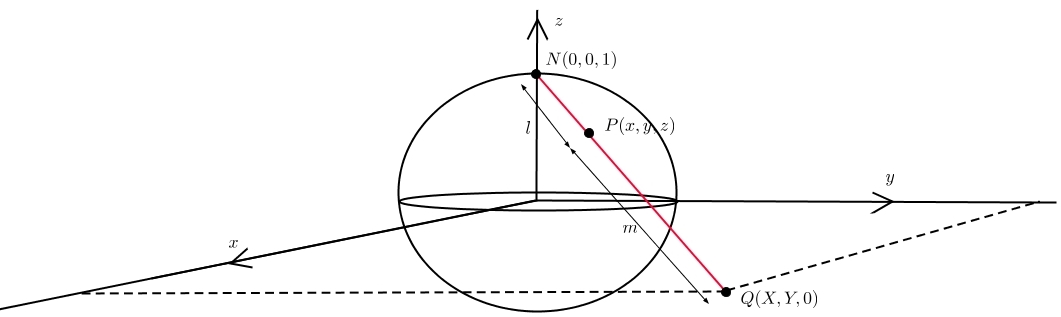
\includegraphics[scale=0.55]{figs/4_1.jpg}
\end{center}
\end{figure}

\noindent By coordinate geometry

\begin{eqnarray*}  
x = \frac{lX + mO}{l+m} = \frac{lX}{l+m}, \\
y = \frac{lY + mO}{l+m} = \frac{lY}{l+m}, \\
z = \frac{l.0+ m.1}{l+m} = \frac{m}{l+m}.
\end{eqnarray*}

\noindent Where O is the position of the origin. This implies that

\begin{eqnarray*}
1-z = \frac{l}{l+m}, \\
x = (1-z)X, \\
y = (1-z)Y.
\end{eqnarray*}

\noindent It is also known that $x^2+ y^2 +z^2 = 1$, so using this relation it is clear that

\begin{eqnarray*}
x^2 + y^2 = 1-z^2 = (1-z) (1+z), \\
(1-z)^2(X^2 +Y^2) = (1-z) (1+z).
\end{eqnarray*}

\noindent If the point $N$ is excluded, i.e. $z \neq 1$ then divide by $(1-z)^2$ to obtain

\begin{equation*} 
X^2 + Y^2 = \frac{1+z}{1-z},
\end{equation*}

\noindent and Rearrange to find

\begin{equation}\label{Ext_Complex_z_in_term_XY} 
z = \frac{X^2 + y^2 - 1}{X^2 + y^2 + 1}.
\end{equation}

Define $\zeta = X+ iY$ and rewrite Eqn.(\ref{Ext_Complex_z_in_term_XY}) to see that

\begin{equation*}
z = \frac{\zeta\bar{\zeta} - 1}{\zeta\bar{\zeta} + 1},
\end{equation*}

\noindent Which implies

\begin{equation*}
1- z = \frac{2}{\zeta\bar{\zeta} + 1}.
\end{equation*}

\noindent So relations for $(x,y,z) \in \mathbb{S}^2 \backslash \{N\}$ have been obtained in terms of $\zeta$, such that

\begin{align}\label{Ext_Complex_xy_interms_zeta}
x + iy & = \zeta (1-z) = \frac{2\zeta}{\zeta\bar{\zeta} + 1}, \\\label{Ext_Complex_z_interms_zeta}
z  & = \frac{\zeta\bar{\zeta} - 1}{\zeta\bar{\zeta} + 1}.
\end{align}

\noindent Hence the points on $\mathbb{S}^2 \backslash \{N\}$ are labelled by complex numbers $\zeta \in \mathbb{C}$. If a point $\zeta = \infty$, called the point at infinity of $\mathbb{C}$, is allowed then the following limits hold

\begin{eqnarray*}
x+ iy = \frac{2/\bar{\zeta}}{1 + 1/\zeta\bar{\zeta}} \rightarrow 0 \text{, as  } \zeta \rightarrow \infty, \\
z = \frac{1- 1/\zeta\bar{\zeta}}{1+ 1/\zeta\bar{\zeta}} \rightarrow 1 \text{, as  } \zeta \rightarrow \infty. 
\end{eqnarray*}

\noindent Then $N = (0,0,1)$ corresponds to $\zeta = \infty$. Thus in this way there is a one to one correspondence between the points of $\mathbb{S}^2$ and the points of the \textit{extended complex plane} $\hat{\mathbb{C}} = \mathbb{C} \cup {\infty}$, which is the usual complex plane with the point at infinity added. Since $\mathbb{S}^2$ has finite surface area, and is therefore called a \textit{compact manifold}, the identification of the points of $\hat{\mathbb{C}}$ with the points of $\mathbb{S}^2$ is called the \textit{compactification} of $\hat{\mathbb{C}}$.

The pair $(\zeta, \bar{\zeta})$ are called the \textit{stereographic coordinates} on $\mathbb{S}^2 \backslash \{N\}$. How are they related to the polar angles $\theta$ and $\phi$? To investigate this write the usual spherical polar coordinates in terms of $\zeta$. First it is known that

\begin{align*}
x & = \sin{\theta}\cos{\phi}, \\
y & = \sin{\theta}\sin{\phi}, \\
z & = \cos{\theta}.
\end{align*}

\noindent So by Eqn.(\ref{Ext_Complex_z_interms_zeta}) it is clear that

\begin{gather*}
z = \cos{\theta} = \frac{\zeta\bar{\zeta} - 1}{\zeta\bar{\zeta} + 1} \\
\zeta\bar{\zeta}\cos{\theta} + \cos{\theta} = \zeta\bar{\zeta} - 1\\
\zeta\bar{\zeta} = \frac{1 + \cos{\theta}}{1 - \cos{\theta}} = \frac{2\cos^2{\left(\theta/2\right)}}{2\sin^2{\left(\theta/2\right)}} \\
\zeta\bar{\zeta} = \cot^2{\left(\theta/2\right)}.
\end{gather*}

\noindent Now use Eqn.(\ref{Ext_Complex_xy_interms_zeta}) to obtain

\begin{gather*}
\sin{\theta}(\cos{\phi} +i \sin{\phi}) = \frac{2\zeta}{\cot^2{\left(\theta/2\right)} + 1 }, \\
2\sin{\left(\theta/2\right)}\cos{\left(\theta/2\right)}e^{i\phi} = 2\zeta \sin^2{\left(\theta/2\right)}, \\
\zeta = e^{i\phi}\cot{\left(\theta/2\right)}. 
\end{gather*}

\noindent This makes sense as if $\zeta = \infty$ then $\theta = 0$ as one would expect. In summary the following coordinate transformations have been constructed

\begin{align}
\vec{n} = (x, y, z) & = (\sin{\theta}\cos{\phi}, \sin{\theta}\sin{\phi}, \cos{\theta}), \\ \label{Ext_Complex_Vec_n}
&
\begin{Huge}
                     = \left( \frac{\bar{\zeta} + \zeta}{\bar{\zeta}\zeta + 1}  ,i\frac{\bar{\zeta} - \zeta}{\bar{\zeta}\zeta + 1}, \frac{\bar{\zeta}\zeta - 1}{\bar{\zeta}\zeta + 1}  \right),
\end{Huge}
\end{align}

\noindent where here $\vec{n}$ is a unit vector in $\mathbb{R}^3$ such that $\vec{n} \cdot \vec{n} = 1$. (ERROR. SHOULD I SHOW THIS)

\subsection{Extension to Minkowskian Sapce-Time}\label{Fractional_Section_Extension_to_Minkowskian}

These results are now extended to Minkowskian space-time to derive an expression for the fractional Linear transformation. Let $\vec{x} = (x,y,z,t)$ be a point on the future null cone with origin $(0,0,0,0)$. Denote the future null cone as $N^{+}$, so that 

\begin{equation*}
N^+ : x^2 + y^2 + z^2 - t^2 = 0 \text{,  for  } t>0,
\end{equation*}

\noindent as all the vectors in the null cone have a Lorentz quadratic form equal to zero by definition. The intersection with the space-like hypersurface $t = \text{const}>0$ is a 2-sphere denoted by 

\begin{equation}\label{Ext_Complex_2Sphere_Definition}
\mathbb{S}^2 (t) : x^2 + y^2 + z^2 = t^2 = \text{const}, 
\end{equation}

\noindent see Fig.(\ref{Ext_Complex_Intersection_Cone_Plane_Fig}). There is a generator of $N^+$ passing through each point of $\mathbb{S}^2 (t)$, they are the null geodesics tangent to $N^+$ and passing through the point $(0,0,0,0)$. Hence the points of $\mathbb{S}^2 (t)$, denoted by $(\theta,\phi)$ or $\zeta$, label the \textit{generators} of $N^{+}$.

\begin{figure}[h!]
\begin{center}
\caption{\textit{Future null cone of Minkowskian space-time. Shown in red is the intersection between the future null cone and the hyperplane $t=\text{const}$. This surface is the sphere in three dimensions from which a stereographic projection was derived earlier.}}
\label{Ext_Complex_Intersection_Cone_Plane_Fig}
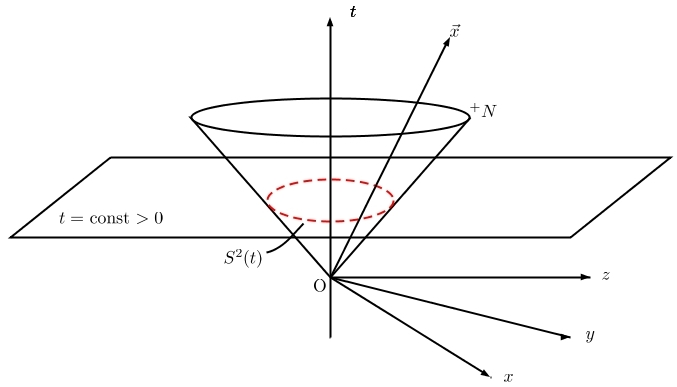
\includegraphics[scale=0.6]{figs/4_5.jpg}
\end{center}
\end{figure}

For every generator and any $t>0$ it is clear that

\begin{equation*}
\left(\frac{x}{t}\right)^2 +\left(\frac{y}{t}\right)^2 +\left(\frac{z}{t}\right)^2 = 1.
\end{equation*}

\noindent This is just the definition of a $2$-sphere, as in Eqn.(\ref{Ext_Complex_2Sphere_Definition}), normalised with respect to a constant $t$. Hence we can write $\vec{x}$ in terms of the coordinate transformation of (\ref{Ext_Complex_Vec_n})

\begin{align}\nonumber
\vec{x} & = t(\sin{\theta}\cos{\phi}, \sin{\theta}\sin{\phi}, \cos{\theta}, 1), \\\label{Ext_Complex_vec_x_relations}
        & = t
\begin{Huge}
\left( \frac{\bar{\zeta} + \zeta}{\bar{\zeta}\zeta + 1}  ,i\frac{\bar{\zeta} - \zeta}{\bar{\zeta}\zeta + 1}, \frac{\bar{\zeta}\zeta - 1}{\bar{\zeta}\zeta + 1},1  \right).
\end{Huge}
\end{align}

\noindent Where a $4^{\text{th}}$ component is included as $\vec{x}$ is an element of Minkowskian space-time. Thus the direction of $\vec{x}$ is determined explicitly by $(\theta,\phi)$ or $\zeta$ as $\vec{x}$ has the same form as the unit vector of Eqn.(\ref{Ext_Complex_Vec_n}). Note that all possible directions of $\vec{x}$ on $N^{+}$ are covered if $\zeta \in \hat{\mathbb{C}}$. Now the Lorentz transformation $\vec{x} \rightarrow \vec{x}'$ is investigated, it takes the form  

\begin{equation*}
\vec{x} \rightarrow \vec{x}' = t'\left( \frac{\bar{\zeta'} + \zeta'}{\bar{\zeta'}\zeta' + 1}  ,i\frac{\bar{\zeta'} - \zeta'}{\bar{\zeta'}\zeta' + 1}, \frac{\bar{\zeta'}\zeta' - 1}{\bar{\zeta'}\zeta' + 1},1  \right).
\end{equation*}

\noindent The null direction $\zeta$ is transformed to the null direction $\zeta'$, where the relation between them must be determined. Construct the matrix $A(\vec{x})$ as in Eqn.(\ref{Special_Matrices_A_first}),

\begin{equation*}
A(\vec{x}) = 
\left(
\begin{array}{ccc}
\frac{2t}{\zeta\bar{\zeta}+1} & & \frac{2t\zeta}{\zeta\bar{\zeta}+1} \\
 & & \\
\frac{2t\bar{\zeta}}{\zeta\bar{\zeta}+1} & & \frac{2t\zeta\bar{\zeta}}{\zeta\bar{\zeta}+1} \\
\end{array}
\right)
=
c_0\left(
\begin{array}{cc}
1           & \zeta \\ 
\bar{\zeta} & \bar{\zeta}\zeta \\ 
\end{array}
\right),
\end{equation*}

\noindent where $c_0 = 2t/(\zeta\bar{\zeta}+1) \in \mathbb{R}^2$. Note that as $\vec{x}$ is a null vector $\det{(A(\vec{x}))} = 0$. Thus the transformed matrix $A(\vec{x}')$ is given similarly as

\begin{equation*}
A(\vec{x}') = 
{c_0}'\left(
\begin{array}{cc}
1           & \zeta' \\ 
\bar{\zeta'} & \bar{\zeta'}\zeta' \\ 
\end{array}
\right).
\end{equation*}

\noindent Now, as in the examples in section (\ref{Special_Linear_Matrices_of_Lorentz}) we determine the special linear matrix $U$ such that

\begin{equation}\label{Ext_Complex_UAU}
A(\vec{x}') = U A(\vec{x}) U^{\dagger}
\end{equation}

\noindent As before, this matrix equation is written component wise as

\begin{equation*}
{c_0}'\left(
\begin{array}{cc}
1           & \zeta' \\ 
\bar{\zeta'} & \bar{\zeta'}\zeta' \\ 
\end{array}
\right)
=
\left(
\begin{array}{cc}
\alpha & \beta \\
\gamma & \delta \\
\end{array}
\right)
{c_0}\left(
\begin{array}{cc}
1           & \zeta \\ 
\bar{\zeta} & \bar{\zeta}\zeta \\ 
\end{array}
\right)
\left(
\begin{array}{cc}
\bar{\alpha} & \bar{\beta} \\
\bar{\gamma} & \bar{\delta} \\
\end{array}
\right).
\end{equation*}

\noindent Then three separate relations between $\zeta$ and $\zeta'$ are obtained

\begin{align}\label{Ext_Complex_zeta_trans_1} 
{c_0}' & = c_0 (\alpha \bar{\alpha} + \alpha \bar{\beta} \zeta + \bar{\alpha} \beta \bar{\zeta} + \beta \bar{\beta} \zeta \bar{\zeta}), \\\label{Ext_Complex_zeta_trans_2} 
{c_0}'\zeta' & = c_0 (\alpha \bar{\gamma} + \alpha \bar{\delta} \zeta + \bar{\gamma} \beta \bar{\zeta} + \beta \bar{\delta} \zeta \bar{\zeta}), \\\label{Ext_Complex_zeta_trans_3} 
{c_0}'\zeta'\bar{\zeta'} & = c_0 (\gamma \bar{\gamma} + \gamma \bar{\delta} \zeta + \bar{\gamma} \delta \bar{\zeta} + \delta \bar{\delta} \zeta \bar{\zeta}). 
\end{align} 

\noindent Using Eqns.(\ref{Ext_Complex_zeta_trans_1}) and (\ref{Ext_Complex_zeta_trans_2}) and factorising to obtain

\begin{equation*}
\zeta' = \frac{{c_0}'\zeta'}{{c_0}'} = \frac{\alpha(\bar{\gamma} + \bar{\delta}\zeta) + \beta \bar{\zeta}(\bar{\gamma} + \bar{\delta}\zeta)}{\alpha(\bar{\alpha} + \bar{\beta}\zeta) + \beta \bar{\zeta}(\bar{\alpha} + \bar{\beta}\zeta)} \\
\end{equation*}

\noindent Thus 

\begin{equation}\label{Extended_Complex_Fractional_Linear_Transformation}
\zeta' = \frac{(\bar{\gamma} + \bar{\delta}\zeta)}{(\bar{\alpha} + \bar{\beta}\zeta)},
\end{equation}

\noindent with $\alpha\delta - \beta\gamma = 1$ as before. This is a \textit{fractional linear transformation} of the extended complex plane $\hat{\mathbb{C}}$. There is a one to one correspondence here between proper, orthochronous Lorentz transformations and fractional linear transformations of the extended complex plane. This is because the matrices $\pm U$ both satisfy Eqn.(\ref{Ext_Complex_UAU}) as in the previous section, but now both matrices give the same transformation as the signs will cancel in the fractional transformation.

\subsection{Fixed points and Their Associated Null Directions}

A given Lorentz transformation is equivalent to known $\alpha$, $\beta$ , $\gamma$ and $\delta$ parameters module a sign and therefore gives an explicit fractional linear transformation. For a given Lorentz transformation a \textit{fixed point} of the corresponding fractional linear transformation corresponds to an invariant null direction. The fixed points $\zeta$ satisfy the relation $\zeta' = \zeta$. Thus from Eq.(\ref{Extended_Complex_Fractional_Linear_Transformation})

\begin{gather}\nonumber
\zeta' = \frac{(\bar{\gamma} + \bar{\delta}\zeta)}{(\bar{\alpha} + \bar{\beta}\zeta)} = \zeta, \\\label{Ext_Complex_fixed_point}
\bar{\beta}\zeta^2 + (\bar{\alpha}- \bar{\delta})\zeta - \bar{\gamma} = 0. 
\end{gather}

\noindent Clearly this is a quadratic equation over the field $\mathbb{C}$, thus it has two roots in general. The non-singular case is when these roots do not coincide, hence a Lorentz transformation does indeed leave two null directions invariant in general.  If Eqn.(\ref{Ext_Complex_fixed_point}) has only one root then the corresponding Lorentz transformation leaves one null direction invariant, this is the singular case.

Consider Eqn.(\ref{Ext_Complex_fixed_point}) again. Divide by $\zeta^2$ to obtain

\begin{equation*}
\bar{\beta} + (\bar{\alpha}- \bar{\delta})\zeta^{-1} - \bar{\gamma}\zeta^{-2} = 0.
\end{equation*}

\noindent Hence $\zeta = \infty$ is a solution of this equation if $\beta = 0$. If $\zeta = \infty$ then $\vec{x}$ is given by $\vec{x} = t(0,0,1,1)$ by Eqn.(\ref{Ext_Complex_vec_x_relations}). Thus it is clear that this corresponds to the null direction $z=t$. Compare this to Example 3, Section (\ref{Special_Linear_Matrices_Example_3}). Here $\beta$ is zero AND the null direction is $z=t$ as expected. If $\zeta = 0$ is a solution to Eqn.(\ref{Ext_Complex_fixed_point}) it is required that $\gamma = 0$, thus $\vec{x} = (0,0,-1,1)$. So it is predicted that a Lorentz transformation with a special linear matrix of the form

\begin{equation*}   
U = 
\left(
\begin{array}{cc}
\alpha & \beta \\
0 & \delta \\
\end{array}
\right),
\end{equation*}   

\noindent will leave the $z=-t$ null direction invariant. The example in section (\ref{Ext_Complex_Ex_end}) illustrates a case where the null direction is found to be $x=\pm t$, due to the form of the matrix $U$. The choice of the components of the matrix $A$ in Eqn.(\ref{Special_Matrices_A_first}) determine which direction is the null direction. The initial choice of $A$ gives special significance to the $z$ component, this of course is arbitrary. In Appendix (\ref{Appendix_Special_Significance_x}), the example in Section (\ref{Special_Linear_Matrices_Example_3}) is repeated for the case when special significance is given to $x$. 

\subsection{Example: Standard Lorentz Transformation}\label{Ext_Complex_Ex_end}

Continuing on from Example 2, section (\ref{Special_Linear_Matrices_Example_2}), where $\alpha$, $\beta$, $\gamma$ and $\delta$ were determined. $\zeta'$ can now be expressed as a fractional linear transformation by Eqn.(\ref{Extended_Complex_Fractional_Linear_Transformation})

\begin{equation*} 
\zeta' = \frac{-\sqrt{\gamma_0 - 1} + \sqrt{\gamma_0 + 1}\zeta}{\sqrt{\gamma_0 + 1} - \sqrt{\gamma_0 - 1}\zeta}.
\end{equation*}

\noindent If the condition $\zeta' = \zeta$ is imposed then

\begin{gather*}
\sqrt{\gamma_0 - 1}(\zeta^2 - 1) = 0, \\
\zeta = \pm 1.
\end{gather*}

In the $\zeta = +1$ case, $\vec{x} = t(1,0,0,1)$ and the invariant direction is $x=t$. Similarly in the $\zeta = -1$ case $\vec{x} = t(-1,0,0,1)$ and the invariant direction is $x = - t$. 



   














\section{Infinitesimal Lorentz Transformations}

There are Lorentz transformations that are small perturbations of the identity transformation and so $U \in SL(2,\mathbb{C})$ has the form

\begin{equation}\label{Infinitesimal_Infinitesimal_Lorentz_Transform_Matrix_U}
U = \pm
\left(
\begin{array}{cc}
1 + \epsilon a & \epsilon b \\
\epsilon c & 1 + \epsilon f \\
\end{array}
\right),
\end{equation}

\noindent where $a,b,c,f \in \mathbb{C}$ and $\epsilon$ is a small real parameter. Here terms of order $\epsilon^2$ will be neglected. As $U \in SL(2,\mathbb{C})$ its determinant is calculated as

\begin{equation*}
\det{(U)} = 1 + O(\epsilon^2).
\end{equation*}

\noindent Using this it is possible to obtain a relation between $f$ and $a$

\begin{eqnarray*}
(1 + \epsilon a)(1 + \epsilon f) - \epsilon^2 b c = 1 + O(\epsilon^2), \\
1 + \epsilon (a +f) = 1 + O(\epsilon^2), \\
\Rightarrow f = -a + O(\epsilon).
\end{eqnarray*}

\noindent Hence 

\begin{equation*}
U =
\left(
\begin{array}{cc}
1 + \epsilon a & \epsilon b \\
\epsilon c & 1 - \epsilon a \\
\end{array}
\right),
\end{equation*}

Now the explicit infinitesimal Lorentz transformations are calculated as in section \ref{Special_Linear_Matrices_of_Lorentz}, by substituting $U$ into

\begin{equation*}
A(\vec{x}') = U A(\vec{x}) U^{\dagger}.
\end{equation*}

\noindent Now writing this out in component form to obtain

\begin{eqnarray*}
\left(
\begin{array}{cc}
t'-z' & x' + iy' \\
x' + iy' & t'+z' \\
\end{array}
\right)
=
\left(
\begin{array}{cc}
1 + \epsilon a & \epsilon b \\
\epsilon c & 1 - \epsilon a \\
\end{array}
\right)
\left(
\begin{array}{cc}
t-z & x + iy \\
x - iy & t+z \\
\end{array}
\right)
\left(
\begin{array}{cc}
1 + \epsilon  \bar{a} & \epsilon \bar{c} \\
\epsilon \bar{b} & 1 - \epsilon \bar{a} \\
\end{array}
\right), \\
=
\left(
\begin{array}{cc}
1 + \epsilon a & \epsilon b \\
\epsilon c & 1 - \epsilon a \\
\end{array}
\right)
\left(
\begin{array}{cc}
(t-z)(1 + \epsilon \bar{a})+\epsilon \bar{b}(x + iy) & (t-z)\epsilon \bar{c}+ (1 - \epsilon \bar{a})(x + iy) \\
(x - iy)(1 + \epsilon \bar{a}) +\epsilon \bar{b} (t+z) & (x - iy)\epsilon \bar{c}+(1 - \epsilon \bar{a})(t+z) \\
\end{array}
\right).
\end{eqnarray*}

\noindent This then implies the three relations

\begin{eqnarray}\label{Infinitesimal_Lorentz_Transform_1}
t'-z' = t-z + \epsilon(a + \bar{a})(t-z) + \epsilon(b + \bar{b})x + i\epsilon(\bar{b} - b)y + O(\epsilon^2), \\\label{Infinitesimal_Lorentz_Transform_2}
t'+z' = t+ z - \epsilon(a + \bar{a})(t+z) + \epsilon (c + \bar{c})x + i \epsilon(c-\bar{c})y + O(\epsilon^2), \\\label{Infinitesimal_Lorentz_Transform_3}
x'+iy' = x+iy + \epsilon(a-\bar{a})(x+iy) + \epsilon(b + \bar{c})t + \epsilon (b-\bar{c})z + O(\epsilon^2).
\end{eqnarray}

\noindent As $a,b,c \in \mathbb{C}$, set 

\begin{equation*}
a = a_1 +ia_2 \text{,  } b = b_1 +ib_2 \text{,  } c = c_1 +ic_2 \text{.} 
\end{equation*}

\noindent Then subbing these into the above equations, eliminating $t$ and $z$ respectively from Eqn.(\ref{Infinitesimal_Lorentz_Transform_1}) and (\ref{Infinitesimal_Lorentz_Transform_2}) and taking real and imaginary parts of Eqn.(\ref{Infinitesimal_Lorentz_Transform_3}) to obtain

\begin{equation}\label{infinitesimal_Matrix_component_wise}
\left(
\begin{array}{c}
x' \\
y'\\
z'\\
t'\\
\end{array}
\right)
=
\left(
\begin{array}{c}
x \\
y\\
z\\
t\\
\end{array}
\right)
+ \epsilon
\left(
\begin{array}{cccc}
0            & -2a_2        & (b_1 - c_1) & (b_1+c_1)\\
2a_2         & 0            & (b_2+c_2)   & (b_2 - c_2) \\
-(b_1 - c_1) & -(b_2 - c_2) & 0           & -2a_1 \\
(b_1 + c_1)  & (b_2-c_2)    & -2a_1       & 0 \\
\end{array}
\right)
\left(
\begin{array}{c}
x \\
y\\
z\\
t\\
\end{array}
\right)
+ O(\epsilon^2).
\end{equation}

\noindent The above $4 \times 4$ matrix will be denoted as $\tensor{L}{^i_j}$, so that Eqn.(\ref{infinitesimal_Matrix_component_wise}) can be written simply as 

\begin{equation}\label{Infinitesimal_Infinitesimal_Lorentz_Transformation}
\bar{x}^i = x^i + \epsilon \tensor{L}{^{i}_{j}} x^j + O(\epsilon^2).
\end{equation}

\noindent Where $\bar{x}^i = (x',y',z',t')$. It is also necessary to check that the Lorentz invariance of the quadratic form still holds. 

\begin{eqnarray*}
{x'}^2 + {y'}^2 + {z'}^2 - {t'}^2 & = x^2 + y^2 + z^2 - t^2 - 4\epsilon a_2 x y + 2 \epsilon(b_1 + c_1)xt \\
                                  & + 2\epsilon (b_1 - c_1)xz + 4 \epsilon a_2 yx + 2\epsilon (b_2 - c_2)yt \\
                                  & + 2 \epsilon (b_2 + c_2)yz - 4\epsilon a_1 zt + 2 \epsilon (c_1 - b_1)zx \\
                                  & -2 \epsilon (c_2 + b_2)zy + 4 \epsilon a_1 tz - 2 \epsilon (c_1 + b_1)tx \\
                                  & -2\epsilon (b_2 - c_2) ty + O(\epsilon^2) \\
                                  & = x^2 + y^2 + z^2 - t^2 + O(\epsilon^2)
\end{eqnarray*}

\noindent Hence this transforamtion is still a Lorentz Transformation if we neglect terms of order $\epsilon^2$.

Consider the time-like world line (SEE FIG pg 5:3)of a particle in Minkowkian space-time $x^i = x^i(s)$. If $s$ is arc length or proper time then $v^i(s) = \frac{dx^i}{ds}$ is the unit tangent(NOT SURE WHY???) vector field. It is clear that $v^i(s)$ must be time-like as $x^i(s)$ is time-like, thus

\begin{equation*}
\eta_{ij} v^i v^j = -1. 
\end{equation*}

\noindent Where $\eta_{ij} - \text{diag}(1,1,1,-1)$ is the metric of minkowskiam space-time. This implies that 

\begin{equation*}
(v^1)^2  + (v^2)^2 + (v^3)^2  - (v^4)^2 = -1.
\end{equation*}

Now consider taking a step along the world line of the particle. Define $\bar{s} = s + \alpha$, where $\alpha$ is some real parameter, so that $v^i (s+\alpha) \vcentcolon = \bar{v}^i(\bar{s})$. Hence we also have

\begin{equation*}
({\bar{v}^1})^2  + ({\bar{v}^2})^2 + ({\bar{v}^3})^2  - ({\bar{v}^4})^2 = -1,
\end{equation*}

\noindent and so $v^i(s)$ and $\bar{v}^i(\bar{s})$ are related by a Lorentz transformation. In particlular $v^i(s+\epsilon)$ and $v^i(s)$ are related by an infinitesimal Lorentz Transformation given by Eqn.(\ref{Infinitesimal_Infinitesimal_Lorentz_Transformation}),

\begin{equation}
v^i(s+\epsilon) = v^i(s) = \epsilon \tensor{L}{^{i}_{j}}(s)v^j (s) + O(\epsilon^2).
\end{equation}

\noindent Rearranging to obtain

\begin{equation}
\frac{v^i(s+\epsilon) - v^i(s)}{\epsilon} = \tensor{L}{^{i}_{j}}(s)v^j (s) + O(\epsilon).
\end{equation}

\noindent Now taking the limit as the infinitesimal step, $\epsilon$ goes to zero to obtain a continuous differentiable equation,

\begin{equation}\label{Infinitesimal_DE_interms_v}
\frac{dv^i}{ds} = \tensor{L}{^{i}_{j}}(s) v^j (s).
\end{equation}

\noindent This equation determines the trajectory of the particle through Minkowskian space-time. In terms of $x$ this is equivalent to

\begin{equation*}
\frac{d^2 x^i}{ds^2} = \tensor{L}{^{i}_{j}}(s) \frac{d x^j}{ds}.
\end{equation*}

It is interesting to write these equations in terms of the particles $3$-velocity given by

\begin{equation*}
\vec{u} = \left( \frac{dx}{dt}, \frac{dy}{dt}, \frac{dz}{dt} \right).
\end{equation*}

\noindent Start by using the chain rule on $v^i$,

\begin{equation*}\label{Infinitesimal_Chain_Rule}
v^i = \frac{dx^i}{ds} = \frac{dx^i}{dt} \frac{dt}{ds} = \left(\frac{dx}{dt},\frac{dy}{dt},\frac{dz}{dt},1\right) \frac{dt}{ds}.
\end{equation*}

\noindent Now determine the first integral of $v^i$, which is equal to $-1$ as $v^i$ is time-like,

\begin{equation*} 
-1 = \eta_{ij} v^i v^j =  \left\{ \left( \frac{d}{dt} \right)^2  + \left( \frac{d}{dt} \right)^2  + \left( \frac{d}{dt} \right)^2 - 1  \right\} \left( \frac{dt}{ds} \right)^2,
\end{equation*} 

\noindent as this is just the scalar product in Minkowskian space-time. Therefore (NOT SURE WHERE THIS COMES FROM)

\begin{equation*}
\frac{dt}{ds} = \gamma (s) \vcentcolon = (1-u^2)^{-1/2},
\end{equation*}

\noindent where $u = |\vec{u}| = \sqrt{\vec{u} \cdot \vec{u}}$. Thus from Eqn.(\ref{Infinitesimal_Chain_Rule})

\begin{equation}\label{infinitesimal_v_interms_gamma}
v^i = \gamma(u) (\vec{u}, 1)
\end{equation}

\noindent It is now conveinient to display Eqn.(\ref{Infinitesimal_DE_interms_v}) as two equations denoting the spacial part and the temproal part, in terms of $\gamma$ and $u$. Again using the chain rule to obtain

\begin{equation*} 
\frac{dt}{ds} \frac{dv^i}{dt} = \tensor{L}{^{i}_{j}}v^j. 
\end{equation*} 

\noindent This then implies that 

\begin{eqnarray}\label{Infinitesimal_gamma_u_1}
\gamma(u) \frac{d}{dt} (\gamma(u) u^{\alpha}) = \tensor{L}{^{\alpha}_{j}} v^j, \\\nonumber
\gamma(u) \frac{d}{dt} \gamma(u) = \tensor{L}{^{4}_{j}} v^j,
\end{eqnarray}

\noindent as $v^i = \gamma(u)(\vec{u},1)$. Here we have used the usual convention that greek indices denote the sum over the spacial indices only, thus $\alpha = 1,2,3$. Now Eqn.(\ref{infinitesimal_v_interms_gamma}) can be used to rewrite the $\tensor{L}{^{i}_{j}}$ coefficients to get

\begin{eqnarray}\label{Infinitesimal_gamma_u_2}
\tensor{L}{^{\alpha}_{j}} v^j = \gamma(u) (\tensor{L}{^{\alpha}_{\beta}} u^{\beta} + \tensor{L}{^{\alpha}_4}) \\ \nonumber
\tensor{L}{^{4}_{j}} v^j = \gamma(u) (\tensor{L}{^{4}_{\alpha}} u^{\alpha0})
\end{eqnarray} 

\noindent where $\tensor{L}{^{4}_{4}} = 0$ from Eqn.(\ref{infinitesimal_Matrix_component_wise}). Putting together Eqns.(\ref{Infinitesimal_gamma_u_1}) and (\ref{Infinitesimal_gamma_u_2}) to obtain differential equations for the spacial and temporal coordinates in terms of the particles $3$-velocity,

\begin{eqnarray*} 
\frac{d}{dt} (\gamma(u) u^{\alpha}) = \tensor{L}{^{\alpha}_{\beta}} u^{\beta} + \tensor{L}{^{\alpha}_{4}}, \\
\frac{d\gamma(u)}{dt} = \tensor{L}{^{4}_{\alpha}} u^{\alpha}.
\end{eqnarray*} 

\noindent These can be written explicitely as four equations

\begin{eqnarray}\label{Infinitesimal_gamma_u_explicit_1}
\frac{d}{dt} (\gamma(u) u^{(1)}) = -2a_2u^{(2)} + (b_1 - c_1)u^{(3)} + b_1 + c_1, \\ \label{Infinitesimal_gamma_u_explicit_2}
\frac{d}{dt} (\gamma(u) u^{(2)}) = 2a_2 u^{(1)} + (b_2 + c_2) u^{(3)} + b_2 - c_2,\\ \label{Infinitesimal_gamma_u_explicit_3}
\frac{d}{dt} (\gamma(u) u^{(3)}) = -(b_1 - c_1) u^{(1)} - (b_2 + c_2 )u^{(2)} - 2a_1,\\ \label{Infinitesimal_gamma_u_explicit_4}
\frac{d\gamma(u)}{dt} = (b_1 + c_1)u^{(1)} + (b_2 - c_2) u^{(2)} - 2a_1 u^{(3)}.
\end{eqnarray}

Now define the $3$-vectors $\vec{P}$ and $\vec{Q}$ such that

\begin{eqnarray*}
\vec{P} = (b_1+c_1,b_2-c_2,-2a_1),
\vec{Q} = (b_2 + c_2, -(b_1 - c_1),-2a_2).
\end{eqnarray*}

It is clear that Eqns.(\ref{Infinitesimal_gamma_u_explicit_1})-(\ref{Infinitesimal_gamma_u_explicit_4}) can be written in terms of $\vec{P}$ and $\vec{Q}$ as follows,

\begin{eqnarray}\label{Infinitesimal_like_Lorentz_force_1}
\frac{d}{dt} (\gamma(u)\vec{u}) = \vec{P} + \vec{u} \times \vec{Q}, \\ \label{Infinitesimal_like_Lorentz_force_2}
\frac{d\gamma}{dt} = \vec{u} \cdot \vec{P}.
\end{eqnarray}

\noindent Note that these expressions look remarkably like the Lorentz force in electromagnetism. It is easily shown that Eqn.(\ref{Infinitesimal_like_Lorentz_force_1}) implies Eqn.(\ref{Infinitesimal_like_Lorentz_force_2}). To see this, first take the scalar product of Eqn.(\ref{Infinitesimal_like_Lorentz_force_1}) with $\vec{U}$.

\begin{eqnarray}\label{Infinitesimal_1_imples_2_calc_1}
\vec{u} \cdot \frac{d}{dt} (\gamma(u)\vec{u}) = \vec{u} \cdot \vec{P} + \vec{u} \cdot (\vec{u} \times \vec{Q}), \\ \label{Infinitesimal_1_imples_2_calc_2}
\gamma \vec{u} \frac{d\vec{u}}{dt} + \vec{u} \cdot \vec{u} \frac{d\gamma}{dt} = \vec{u} \cdot \vec{P},
\end{eqnarray}

\noindent by using the product rule and as the scalar product of the cross product with a repeated vector is zero in the third term. The quantity $\gamma$ is known in terms of $u$, so it is possible to write the derivative in the first term as a derivative of $\gamma$ as follows,

\begin{eqnarray*} 
\gamma^{-2} = 1 - u^{2} = 1- \vec{u} \cdot \vec{u}, \\
\Rightarrow -2 \gamma^{-3} \frac{d\gamma}{dt} = - 2 \vec{u} \cdot \frac{d \vec{u}}{dt}.
\end{eqnarray*}

\noindent Subbing this result back into Eqn.(\ref{Infinitesimal_1_imples_2_calc_2}) to obtain

\begin{eqnarray*} 
\gamma \gamma^{-3} \frac{d\gamma}{dt} + u^2 \frac{d\gamma}{dt} = \vec{u} \cdot \vec{P}, \\
(\gamma^{-2} + u^2) \frac{d\gamma}{dt} = \vec{u} \cdot \vec{P}.
\end{eqnarray*} 

Therefore

\begin{equation*}
\frac{d\gamma}{dt} =  \vec{u} \cdot \vec{P},
\end{equation*}

and so it is shown that Eqn.(\ref{Infinitesimal_like_Lorentz_force_2}) is a generalization of Eqn.(\ref{Infinitesimal_like_Lorentz_force_1}) and contains no new information. 

The dependance of the $3$-force acting on a particle as shown by Eqn.(\ref{Infinitesimal_like_Lorentz_force_1}), depends in general on the particles $3$-velocity $\vec{u}$ in a special way, in order to be compatible with Special Relativity. Thus in particular \textit{the Lorentz $3$-force acting on a particle of rest mass $m$ and charge $q$ must depend upon $\vec{u}$ as in Eqn.(\ref{Infinitesimal_like_Lorentz_force_1}) to be compatible with special Relativity.} So the Lorentz force of electromagnetism is a special case of the a charged particle moving through Minkowskian space-time along a world-line of infiniteimal Lorentz transformations. In this case, make the identifications

\begin{equation}\label{Infinitesimal_P_Q_interms_E_B} 
\vec{P} = \frac{q}{m} \vec{E} \text{, and  } \vec{Q} = \frac{q}{m}\vec{B},
\end{equation} 

\noindent where $\vec{E}$ is the external electric field and $\vec{B}$ is the external magnetic field in which the particle is moving. Then Eqn.(\ref{Infinitesimal_like_Lorentz_force_1}) takes the familiar form

\begin{equation*}
m \frac{d}{dt} (\gamma(u) \vec{u}) = q(\vec{E} + \vec{u} \times \vec{B}).
\end{equation*}

\noindent Or in the case of a slow moving particle $\gamma \approx 1$ and 

\begin{equation*}  
m \vec{a} = q (\vec{E} + \vec{u} \times \vec{B}).
\end{equation*}  

\subsection{Fractional Linear Transformations of the Infinitesimal Linear Transformation}

Recall that the fractional linear transformation constructed in section (\ref{Section_Stereographic_Extended_Complex}) had a one to one correspondence with proper orthochronous Lorentz transforamtions, and the fixed points of the fractional transformation corresponded to null directions of the Lorentz transformation. As in Eqn.(\ref{Extended_Complex_Fractional_Linear_Transformation}), section (\ref{Section_Stereographic_Extended_Complex}) construct the fractional linear transformation of the special linear $(SL(2, \mathbb(C)))$ matrix $U$ for the infinitesimal Lorentz transformation given in Eqn.(\ref{Infinitesimal_Infinitesimal_Lorentz_Transform_Matrix_U}). It is found to be

\begin{equation*}   
\zeta' = \frac{\zeta + \epsilon(\bar{c} - \bar{a}\zeta) + O(\epsilon^2)}{1 + \epsilon(\bar{a} + \bar{b} \zeta) + O(\epsilon^2)}.
\end{equation*}

\noindent Then the fixed points are given when $\zeta' = \zeta$, which implies,

\begin{eqnarray}\nonumber
\epsilon \bar{b} \zeta^2 + (\epsilon \bar{a} + \epsilon \bar{a})\zeta - \epsilon \bar{c} = O(\epsilon^2), \\ \label{Infinitesimal_fixed_point_quadratic}
\Rightarrow \bar{b} \zeta^2 + 2 \bar{a} \zeta - \bar{c} = O(\epsilon).
\end{eqnarray}

\noindent Of interest here are the singular Lorentx transforamtions, so it is required that the roots of this quadratic are the same. Thus the usual discriminant is set to zero,

\begin{equation*} 
4 {\bar{a}}^2 + 4 \bar{b} \bar{c} = 0.
\end{equation*} 

\noindent Therefore,

\begin{equation*}
{\bar{a}}^2 +  \bar{b} \bar{c} \Leftrightarrow a^2 + bc = 0.
\end{equation*}

\noindent Write these equations out explicly and equate real and imaginary coefficients to obtain

\begin{eqnarray}\label{Infinitesimal_discriminant_relation_1}
a_1^2 = a_2^2 + b_1 c_1 - b_2 c_2 = 0, \\\label{Infinitesimal_discriminant_relation_2}
2a_1 a_2 + b_2 c_1 + b_1 c_2 = 0.
\end{eqnarray}

It is interesting to write these equations in terms of the electric and magnetic vectors, namely $\vec{E} = (E^1, E^2, E^3)$ and $\vec{B} = (B^1,B^2,B^3)$. The relation between the $a$,$b$ and $c$ and the $\vec{B}$ and $\vec{E}$ coefficients comes from Eqn.(\ref{Infinitesimal_P_Q_interms_E_B}), where the factor $q/m$ has been suppressed for conveinience. 

\begin{eqnarray}\label{Infinitesimal_abc_interms_EB_1}
a_1 = -\frac{1}{2} E^3 \text{,  } b_2 = \frac{1}{2}(E^2 + B^1) \text{,  } c_1 = \frac{1}{2} (E^1 + B^2) \text{,  } \\\label{Infinitesimal_abc_interms_EB_2}
a_2 = -\frac{1}{2} B^3 \text{,  } b_1 = \frac{1}{2} (E^1 - B^2) \text{,  } c_2  = \frac{1}{2} (B^1 - E^2). 
\end{eqnarray}

\noindent So Eqn.(\ref{Infinitesimal_discriminant_relation_1}) implies

\begin{eqnarray*}
\frac{1}{4} {(E^3)}^2 - \frac{1}{4} {(B^3)}^2 + \frac{1}{4} ({(E^1)}^2 - {(B^2)}^2) + \frac{1}{4} ({(E^2)}^2 - {(B^1)}^2) = 0,
\Rightarrow {(E^1)}^2 + {(E^2)}^2 + {(E^3)}^2 = {(B^1)}^2 + {(B^2)}^2 + {(B^3)}^2.
\end{eqnarray*}

\noindent Thus it is clear that

\begin{equation}\label{Infinitesimal_Pure_Rad_Cond_1}
{|\vec{E}|}^2 = {|\vec{B}|}^2
\end{equation}

\noindent Similarly, Eqn.(\ref{Infinitesimal_discriminant_relation_2}) implies

\begin{eqnarray*}
\frac{1}{2} E^3 B^3 + \frac{1}{4} (E^1E^2 + E^1B^1 + E^2B^2 + B^1B^2) \\
 +  \frac{1}{4} (-E^1E^2 + E^1B^1 + E^2B^2 - B^1B^2) = 0, \\
\Rightarrow E^3B^3 + E^1B^1 + E^2B^2 = 0.
\end{eqnarray*}

\noindent So it is shown that

\begin{equation}\label{Infinitesimal_Pure_Rad_Cond_2}
\vec{E} \cdot \vec{B} = 0.
\end{equation}

\noindent The above Eqns.(\ref{Infinitesimal_Pure_Rad_Cond_1}) and (\ref{Infinitesimal_Pure_Rad_Cond_2}) are the (Lorentz invariant) conditions that the electromagnetic field in which the charged particle is moving is a pure radiation field. Thus in conclusion, \textit{if the world line of the charged particle is generated by infinitesimal singular Lorentz transformations then the particles moving in a pure radiation electromagnetic field.} (CASE WHERE ITS A PLAVE WAVE WORTH DOING???)

\subsection{Pure Radiation Field Conditions in Minkowskian Space-Time}

Eqns.(\ref{Infinitesimal_Pure_Rad_Cond_1}) and (\ref{Infinitesimal_Pure_Rad_Cond_2}) are the pure radiation field conditions in physical space, ${\mathbb{R}}^2$. It is also interesting to see what form these equations take in Minkowskian space-time. To do this, solve the quadratic equation in Eqn.(\ref{Infinitesimal_fixed_point_quadratic}) for the case where the roots coincide, to find the single fixed point of the system. It is clear that 

\begin{equation*}
\zeta = - \frac{\bar{a}}{\bar{b}},
\end{equation*}

\noindent is the fixed point. Now determine the corresponding null direction $k^i$. (HOW DID WE DO THIS???)

\begin{equation*}
k^i = (\bar{\zeta} + \zeta,i(\bar{\zeta} - \zeta),\bar{\zeta}\zeta - 1,\bar{\zeta}\zeta + 1).
\end{equation*}

\noindent Now relate $k^i$ to $\tensor{L}{_i_j} = \eta_{ij} \tensor{L}{^k_j}$. From the relations in (\ref{Infinitesimal_abc_interms_EB_1}) and (\ref{Infinitesimal_abc_interms_EB_2}) it is clear that

\begin{equation*}  
L_{ij} = 
\frac{q}{m}
\left(
\begin{array}{cccc}
0    & B^3  & -B^2 & E^1 \\
-B^3 & 0    & B^1  & E^2 \\
B^2  & -B^1 & 0    & E^3 \\
-E^1 & -E^2 & -E^3 & 0   \\
\end{array}
\right)
=
-(L_{ij}).
\end{equation*}

\noindent The dual of this quantity is defined by

\begin{equation*}
^*L_{ij} = \frac{1}{2} \epsilon_{ijkl} L^{kl},
\end{equation*}

\noindent where $\epsilon_{ijkl}$ is the Levi-Civita permutation symbol in 4 dimensions. 
  












\section{Acknowledgements}
 
\begin{thebibliography}{10}
%\bibitem{CPT}
%Hilary Greaves and Terugi Thomas - ``The CPT Theorem" - April 2012, \url{http://arxiv.org/abs/1204.4674}
\end{thebibliography}

\end{document}
